\documentclass[11pt,a4paper]{article}

\usepackage[utf8]{inputenc}
\usepackage[T1]{fontenc}
\usepackage[spanish,es-nodecimaldot]{babel}
\usepackage{lmodern}
\usepackage{geometry}
\usepackage{graphicx}
\usepackage{booktabs}
\usepackage{array}
\usepackage{tabularx}
\usepackage{longtable}
\usepackage{float}
\usepackage{subcaption}
\usepackage{amsmath}
\usepackage{xcolor}
\usepackage{microtype}
\usepackage{setspace}
\usepackage{enumitem}
\usepackage{fancyhdr}
\usepackage[numbers,sort&compress]{natbib}
\usepackage[hidelinks]{hyperref}

\geometry{top=2.1cm,bottom=2.2cm,left=2.25cm,right=2.25cm}
\setstretch{1.22}
\setlength{\parindent}{1.15em}
\setlength{\parskip}{0.28em}
\setlength{\headheight}{14pt}
\setlength{\emergencystretch}{2em}
\setlist{nosep,leftmargin=1.6em}
\graphicspath{{figures/}{../../../reports/firts-phase/images/}}
\captionsetup{font=small,labelfont=bf}
\hypersetup{
  pdftitle={Doctor Maíz — Informe de Etapa 2},
  pdfauthor={Josias Abner Rivas Fuentes, David Alejandro Deras Cerros, Elmer Edenilson Rosales Molina}
}

\pagestyle{fancy}
\fancyhf{}
\fancyhead[L]{Doctor Maíz}
\fancyhead[R]{Etapa 2}
\fancyfoot[C]{\thepage}
\renewcommand{\headrulewidth}{0.3pt}

\begin{document}

\begin{titlepage}
  \thispagestyle{empty}
  \begin{center}
    \includegraphics[width=0.20\textwidth]{logo_ues.png}\\[0.8cm]
    {\Large\bfseries UNIVERSIDAD DE EL SALVADOR}\\[0.2cm]
    {\large FACULTAD DE INGENIERÍA Y ARQUITECTURA}\\[0.15cm]
    {\large ESCUELA DE INGENIERÍA DE SISTEMAS INFORMÁTICOS}\\[1.25cm]

    {\LARGE\bfseries DOCTOR MAÍZ}\\[0.3cm]
    {\Large Clasificación de enfermedades y deficiencias\\nutricionales en hojas de maíz}\\[0.75cm]
    {\LARGE\bfseries INFORME DE ETAPA 2}\\[0.25cm]
    {\large Optimización, evaluación final y prototipo funcional}\\[1.1cm]

    \begin{tabular}{ll}
      \textbf{Josias Abner Rivas Fuentes} & RF20010 \\
      \textbf{David Alejandro Deras Cerros} & DC19019 \\
      \textbf{Elmer Edenilson Rosales Molina} & RM20001 \\
    \end{tabular}

    \vfill
    {\large San Salvador, El Salvador}\\[0.15cm]
    {\large Septiembre de 2026}
  \end{center}
\end{titlepage}

\pagenumbering{roman}
\section*{Resumen}
\addcontentsline{toc}{section}{Resumen}

Esta segunda etapa parte del clasificador obtenido en la etapa anterior y se
concentra en los problemas que quedaron abiertos: el bajo rendimiento de
potasio, el desbalance, el sesgo laboratorio/campo, la selección del modelo y
una evaluación final que no reutilizara el test histórico. Se reconstruyó la
publicación ampliada del dataset, se verificaron 33\,437 archivos y se
eliminaron cuatro duplicados exactos. El corpus definitivo contiene 33\,433
imágenes de nueve clases, con un holdout nuevo de 5\,015 fotografías congelado
antes de modelar y fingerprint
\texttt{c44de0783d3c3f88ef6151eaa75536d1020f5b208327419c4cb7f3ac459d3892}.

Por ausencia de GPU, los experimentos nuevos utilizaron backbones ImageNet
congelados y una cabeza logística entrenada sobre sus embeddings; no se
presentan como fine-tuning end-to-end. Optuna ejecutó 30 trials sobre
EfficientNet-B0 y podó 13. La mejor configuración elevó el macro-F1 de
validación de la cabeza baseline de 0.7799 a 0.8887, principalmente al usar
balanceo por raíz cuadrada, una tasa menor y penalización L2.
EfficientNet-B0 superó a ShuffleNetV2-x1.0, MobileNetV3 Small y FastViT-T8 como
modelo individual. Los errores fueron suficientemente distintos para que el
weighted soft voting mejorara hasta 0.9202 en validación, con pesos aprendidos
sin consultar el holdout.

En cinco folds, el ensemble obtuvo macro-F1 medio de 0.9097 y desviación 0.0090.
La evaluación única del holdout produjo 0.9537 de accuracy, 0.9012 de precision
macro, 0.9092 de recall macro, 0.9035 de macro-F1 y 0.9537 de F1 ponderado.
Potasio mejoró de forma orientativa desde el F1 histórico 0.62 hasta 0.6706,
pero siguió siendo la clase más débil: 28 de sus 36 errores terminaron en
nitrógeno. Fairness encontró las mayores brechas por clase (0.3206 de F1) y
fuente (0.3151); además, roya obtuvo recall 1.0 en 322 imágenes de laboratorio
y 0.3125 en solo 16 de campo, una señal importante aunque de soporte pequeño.

Grad-CAM y LIME se aplicaron a casos finales, incluidos un error de alta
confianza y una deficiencia nutricional. La demo ejecutable genera Top-3,
confianza, latencia y advertencia sobre una imagen real. También se verificó la
aplicación React Native con EfficientNet-Lite0 TFLite, inferencia offline y
rechazo fuera de dominio: typecheck y 276 pruebas aprobaron. El endpoint y el
APK no estuvieron disponibles en la comprobación final, por lo que el
prototipo es funcional e integrado, pero no recibe puntuación completa de
despliegue público.

\noindent\textbf{Palabras clave:} clasificación foliar, maíz, Optuna, ensemble,
validación cruzada, fairness, interpretabilidad, inferencia móvil.

\clearpage
\tableofcontents
\clearpage
\listoffigures
\clearpage
\listoftables
\clearpage

\pagenumbering{arabic}
\section{Introducción}

\subsection{Punto de partida de la Etapa 1}

La primera etapa dejó un resultado favorable, pero también un problema bastante
claro. Los tres modelos ligeros superaron la meta de macro-F1 de 0.85:
EfficientNet-B0 alcanzó 0.9146, ShuffleNetV2-x1.0 obtuvo 0.9030 y
EfficientNet-Lite0 llegó a 0.8951. La diferencia entre ellos no estaba tanto en
reconocer roya, hojas sanas o necrosis letal, sino en las clases con menos
ejemplos. \texttt{potassium\_deficiency} tenía solamente 266 imágenes y su F1
bajó hasta 0.62 con EfficientNet-B0, 0.54 con ShuffleNet y 0.49 con
EfficientNet-Lite0. El modelo podía acertar casi siempre en el conjunto
completo y, al mismo tiempo, fallar justo en la clase que más necesitaba
mejorar.

La matriz de confusión de aquella etapa mostró que las deficiencias de
nitrógeno, fósforo y potasio compartían parte de sus errores. También aparecía
una confusión menor entre mancha gris y tizón norteño. Las explicaciones LIME y
Grad-CAM aportaron otra advertencia: a veces la red miraba la hoja y aun así se
equivocaba, pero en imágenes de laboratorio también podía aprovechar un fondo
uniforme que no estaría presente en una parcela. La confianza alta tampoco
garantizaba una decisión correcta. Esos hallazgos hicieron insuficiente
limitarse a entrenar más épocas o escoger el mayor valor de accuracy.

Había además un problema de evaluación. El conjunto llamado \emph{test} había
sido consultado durante comparaciones, exportaciones y verificaciones
posteriores. Sus métricas siguen siendo útiles como registro histórico, pero ya
no representan una prueba ciega. Presentarlas otra vez como resultado final
habría dado una precisión metodológica que el experimento no tenía.

\subsection{Alcance de la Etapa 2}

La segunda etapa responde a esos puntos con un protocolo nuevo. Primero se
reconstruyó el corpus desde la publicación completa, se verificó cada archivo y
se retiraron duplicados exactos antes de dividir. Luego se congeló un holdout
nuevo de 5\,015 imágenes, sin emplearlo para elegir arquitectura,
hiperparámetros ni pesos del ensemble. La selección trabajó únicamente con
entrenamiento y validación; el holdout se abrió una vez al final.

La máquina disponible no expuso una GPU CUDA. Para no reemplazar un experimento
real por cifras estimadas, se congelaron backbones preentrenados en ImageNet y
se optimizó sobre sus embeddings una cabeza lineal de pérdida logística. Esto
no equivale al ajuste fino \emph{end-to-end} empleado en la Etapa 1. Sí permite
comparar cuatro representaciones modernas sobre las 33\,433 imágenes únicas,
ejecutar 30 trials de Optuna, probar soft voting, repetir cinco folds y evaluar
el holdout completo en CPU. La restricción cambia la pregunta experimental:
se mide qué tan separables son las nueve clases con cada representación
preentrenada y una cabeza común optimizada. El informe conserva esa distinción
cada vez que compara con el baseline histórico.

También se revisó el producto que rodea al clasificador. La aplicación móvil
captura o selecciona una foto, ejecuta un modelo TFLite local, calcula
confianza y rechazo fuera de dominio, guarda el diagnóstico sin depender de
conectividad y permite sincronizar correcciones. Su modelo embarcado pertenece
a la línea histórica EfficientNet-Lite0; no se sustituyó silenciosamente por el
modelo experimental de esta etapa. La demo incluida aquí ejecuta la selección
de Etapa 2 sobre una imagen real y deja una salida reproducible, mientras la
inspección de la aplicación confirma que existe una ruta móvil completa.

El objetivo no fue acumular arquitecturas. EfficientNet-B0 y ShuffleNet
continuaron por su papel en la etapa anterior; MobileNetV3 Small añadió una
alternativa diseñada para dispositivos; FastViT-T8 permitió contrastar una
arquitectura híbrida reciente. EfficientNet-B4, GhostNetV2 y otros nombres
registrados en el código no aparecen como resultados porque no tuvieron una
corrida completa en este protocolo. Separar lo implementado de lo evaluado
evita convertir el catálogo de modelos en evidencia que no existe.

La lectura final se concentra en cambios observables: cuánto aportó el tuning,
si los modelos cometieron errores distintos, si el ensemble justificó su costo,
qué variación hubo entre folds, qué ocurrió con potasio y qué brechas aparecieron
entre clases, fuentes, resolución, nitidez y entornos de captura. La última
parte traslada esos hallazgos a decisiones de uso. Doctor Maíz puede orientar
una inspección; no identifica con certeza una causa agronómica ni prescribe por
sí solo una aplicación de insumos.

\section{Objetivos}

\subsection{Objetivo general}

Optimizar y evaluar el clasificador de Doctor Maíz sobre el corpus actualizado,
con un protocolo reproducible que permita seleccionar una alternativa
experimental, medir su comportamiento por clase y condición de captura, y
comprobar su integración en un prototipo de diagnóstico asistido.

\subsection{Objetivos específicos}

\begin{enumerate}
  \item Reconstruir el dataset definitivo de la etapa, validar sus archivos,
  eliminar duplicados exactos y congelar una división que mantenga separado el
  holdout final.

  \item Optimizar una cabeza clasificadora sobre EfficientNet-B0 mediante
  búsqueda TPE y pruning con Optuna, usando macro-F1 de validación como función
  objetivo y sin consultar el holdout.

  \item Comparar EfficientNet-B0, ShuffleNetV2-x1.0, MobileNetV3 Small y
  FastViT-T8 bajo el mismo preprocesamiento, partición y configuración de
  cabeza, incluyendo calidad, cantidad de parámetros y latencia CPU del
  backbone.

  \item Medir complementariedad de errores y contrastar el mejor modelo
  individual con soft voting uniforme y ponderado. Los pesos deben aprenderse
  únicamente en validación.

  \item Estimar la estabilidad de la selección con cinco folds estratificados
  por clase y entorno, y efectuar una sola evaluación sobre el holdout
  congelado con métricas globales y por clase.

  \item Revisar el principal cuello de botella de la Etapa 1,
  \texttt{potassium\_deficiency}, cuantificando sus confusiones con nitrógeno,
  fósforo y las demás categorías.

  \item Explicar casos finales con Grad-CAM y LIME, y describir brechas de
  precision, recall y F1 asociadas con clase, laboratorio/campo, fuente,
  resolución y nitidez.

  \item Verificar el flujo real de la aplicación móvil y producir una demo
  ejecutable que muestre entrada, preprocesamiento, Top-3, confianza, latencia
  y advertencia de uso.

  \item Traducir las limitaciones encontradas en condiciones de uso,
  recomendaciones para extensionistas y propuestas concretas de política
  pública, sin presentar beneficios no medidos.
\end{enumerate}

Estos objetivos combinan tres niveles que en la primera etapa todavía estaban
separados: calidad estadística, comportamiento bajo condiciones distintas y
operación dentro de una herramienta usable. Una mejora pequeña en macro-F1 no
compensa una caída fuerte en campo; del mismo modo, una aplicación bien
diseñada no corrige una clase minoritaria mal reconocida. La selección final se
lee con las tres dimensiones.

\section{Dataset actualizado y protocolo experimental}

\subsection{Qué cambió desde la Etapa 1}

La Etapa 1 trabajó con 31\,622 imágenes. Después se añadieron ejemplos a las
clases que habían quedado más cortas: mancha gris y las tres deficiencias
nutricionales. La publicación completa consultada para esta etapa contenía
33\,437 archivos distribuidos en nueve clases \citep{huggingface2026maize}.
Todos se abrieron, se normalizó su orientación EXIF y se calculó SHA-256,
resolución y varianza del Laplaciano como indicador descriptivo de nitidez.
No hubo imágenes ilegibles. Cuatro archivos de hojas sanas repetían exactamente
el contenido de otro archivo y se eliminaron antes de dividir. El corpus
experimental quedó en 33\,433 imágenes únicas.

Esta secuencia explica cifras que antes podían parecer contradictorias.
31\,622 corresponde al corpus de la Etapa 1; 33\,437 es el número de archivos
de la publicación ampliada; 33\,433 es el total utilizado aquí después de la
deduplicación. La cifra 33\,438 que aparecía en una versión de la auditoría no
coincidió con el dataset descargado ni con su manifiesto y por eso no se
conservó como resultado.

\begin{table}[H]
  \centering
  \caption{Composición por clase antes y después de la ampliación. La fuente es
  el manifiesto generado, no una transcripción manual.}
  \label{tab:dataset-e1-e2}
  \small
  \begin{tabular}{lrrr}
\toprule
\textbf{Clase} & \textbf{Etapa 1} & \textbf{Etapa 2} & \textbf{Cambio} \\
\midrule
Roya común & 2~256 & 2~256 & +0 \\
Gusano cogollero & 4~857 & 4~857 & +0 \\
Mancha gris & 1~119 & 1~930 & +811 \\
Sana & 8~744 & 8~740 & -4 \\
Necrosis letal & 6~415 & 6~415 & +0 \\
Def. nitrógeno & 523 & 846 & +323 \\
Tizón norteño & 6~830 & 6~830 & +0 \\
Def. fósforo & 612 & 938 & +326 \\
Def. potasio & 266 & 621 & +355 \\
Total & 31~622 & 33~433 & +1811 \\
\bottomrule
\end{tabular}

\end{table}

El incremento no fue uniforme. Potasio pasó de 266 a 621 imágenes y fósforo de
612 a 938; nitrógeno llegó a 846. Mancha gris recibió la mayor ampliación
absoluta entre las clases problemáticas, de 1\,119 a 1\,930. Aun así, la clase
sana conserva 8\,740 imágenes, más de catorce veces el soporte de potasio. La
ampliación reduce el extremo del desbalance, pero no lo elimina.

\subsection{Composición y procedencia}

El manifiesto conserva catorce identificadores de fuente obtenidos del nombre
versionado de cada archivo. Las colecciones más grandes son
\texttt{maize\_africa}, \texttt{multi\_desease},
\texttt{maize\_desease\_v1.1}, \texttt{corn\_leaf\_roboflow} y
\texttt{cropdg}. No existe un identificador de finca, municipio, dispositivo o
campaña de captura. Por eso «fuente» permite detectar diferencias entre
colecciones, pero no medir generalización geográfica en El Salvador.

La etiqueta de entorno separa 3\,551 imágenes de laboratorio y 29\,882 de
campo. Su distribución está muy lejos de ser factorial: roya común concentra
2\,150 imágenes de laboratorio y 106 de campo; mancha gris tiene 513 y 1\,417;
tizón norteño 888 y 5\,942. Las otras seis clases no poseen ejemplos de
laboratorio. Esta asimetría importa más que el total global. Si el grupo de
laboratorio obtiene otro F1, la diferencia puede deberse tanto al fondo como a
las clases que lo componen.

\begin{figure}[H]
  \centering
  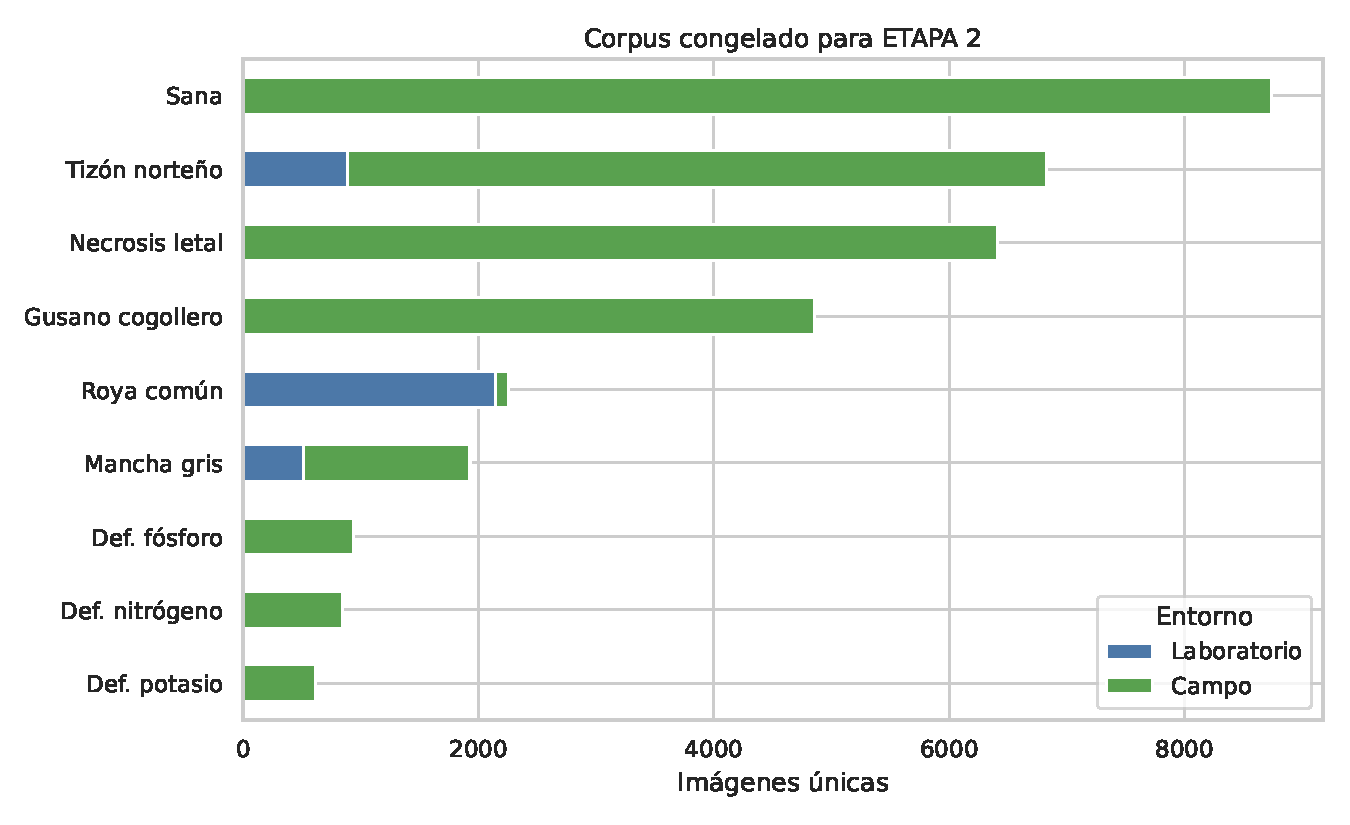
\includegraphics[width=0.90\textwidth]{dataset_distribution.pdf}
  \caption{Distribución del corpus único por clase y entorno. Las deficiencias
  ampliaron su soporte, pero siguen siendo minoritarias y exclusivamente de
  campo en los metadatos disponibles.}
  \label{fig:dataset-distribution}
\end{figure}

La Figura~\ref{fig:dataset-distribution} deja ver dos riesgos. El primero es el
peso de la clase sana y de necrosis letal frente a las deficiencias. El segundo
es que «laboratorio» funciona casi como una pista de clase. Esto impide
interpretar una diferencia global laboratorio/campo como efecto puro del
entorno y obliga a acompañarla con comparaciones dentro de las tres clases que
sí aparecen en ambos grupos.

\subsection{Prevención de fugas y división}

La deduplicación se hizo antes del muestreo. Cada fila contiene ruta relativa,
clase, índice de clase, entorno, fuente, ancho, alto, megapíxeles, indicador de
blur y SHA-256. El fingerprint del conjunto completo se calculó ordenando las
rutas y concatenando ruta, clase, entorno y hash. El valor resultante es:

\begin{center}
\small\ttfamily
c44de0783d3c3f88ef6151eaa75536d1020f5b208327419c4cb7f3ac459d3892
\end{center}

Se reservaron 5\,015 imágenes (15\%) como holdout con semilla 4202. El 85\%
restante se dividió en 23\,403 imágenes de entrenamiento y 5\,015 de
validación, utilizando semilla 42. Ambos cortes se estratificaron por la
combinación clase--entorno. El archivo \texttt{holdout.lock.json} se creó antes
de extraer características y guarda el fingerprint, el hash del CSV de holdout
y la regla de no consultar sus etiquetas durante selección.

El conjunto histórico llamado test no se reutilizó como prueba final. Esa
decisión sacrifica comparabilidad directa con la Etapa 1, pero recupera una
interpretación limpia: la evaluación final responde a decisiones fijadas sin
haber visto esas 5\,015 etiquetas. Los resultados de ambas etapas se comparan
más adelante como referencias sobre corpus y protocolos distintos, no como
una prueba controlada de superioridad.

\subsection{Preprocesamiento y métricas}

Las imágenes se corrigieron según EXIF, se convirtieron a RGB, se redimensionaron
a la entrada nativa de cada backbone y se normalizaron con media y desviación
de ImageNet. El redimensionamiento directo no conserva la relación de aspecto;
es una limitación deliberadamente visible del protocolo. Cada foto se decodificó
una vez durante la extracción conjunta, y FastViT recibió 256 píxeles mientras
los otros backbones recibieron 224.

La métrica de selección fue macro-F1, porque concede el mismo peso a potasio y
a la clase sana. También se guardaron accuracy, precision macro, recall macro
y F1 ponderado. Accuracy permite continuidad con la etapa anterior; F1
ponderado describe el volumen total; macro-F1 evita que cualquiera de esas dos
lecturas oculte las clases pequeñas. Para fairness se calcularon las mismas
métricas dentro de grupos, pero sus brechas se reportan como diferencias
descriptivas y no como causalidad.

\section{Optimización del clasificador}

\subsection{Baseline de referencia}

EfficientNet-B0 se mantuvo como punto de partida porque había obtenido el mejor
macro-F1 de la Etapa 1. En la corrida nueva no se volvió a entrenar toda la red:
se retiró su clasificador, se congelaron los 4\,007\,548 parámetros del
backbone ImageNet y se extrajo un vector de 1\,280 características por imagen.
Sobre esos vectores se ajustó una regresión logística multiclase incremental
con SGD.

El baseline interno de esta etapa usa $\alpha=10^{-4}$, tasa constante 0.01,
penalización L2, batch 256, promedio de pesos, normalización L2 de embeddings y
20 épocas. No debe confundirse con el EfficientNet-B0 end-to-end histórico. El
primero sirve para aislar el efecto del tuning bajo el nuevo protocolo; el
segundo conserva la referencia de 0.9146 macro-F1 sobre el corpus y test de la
Etapa 1.

\subsection{Espacio de hiperparámetros}

Optuna se eligió porque el muestreador TPE usa los trials previos para concentrar
la búsqueda y porque el pruning puede detener combinaciones que ya muestran un
macro-F1 poco competitivo \citep{akiba2019optuna}. Se ejecutaron 30 trials con
semilla 42. El objetivo fue macro-F1 en las 5\,015 imágenes de validación; el
holdout no participó.

La búsqueda cubrió $\alpha$ entre $10^{-6}$ y $10^{-3}$ en escala logarítmica,
tasa inicial entre $3\times10^{-4}$ y $5\times10^{-2}$ también logarítmica,
penalización L2 o elastic net, proporción L1 entre 0 y 0.5 cuando correspondía,
batch de 128, 256 o 512, promedio de pesos activado o no, embeddings con o sin
normalización L2 y potencia de balanceo 0, 0.5 o 1. Esta última transforma los
pesos inversos de clase: cero no rebalancea, 0.5 aplica raíz cuadrada y uno usa
la inversa completa.

\begin{table}[H]
  \centering
  \caption{Configuración del baseline interno y combinación seleccionada por
  Optuna.}
  \label{tab:tuning-config}
  \small
  \begin{tabular}{lcc}
\toprule
\textbf{Hiperparámetro} & \textbf{Baseline} & \textbf{Mejor valor} \\
\midrule
alpha & 0.0001 & 4.2836449125618075e-06 \\
eta0 & 0.01 & 0.0006059127453715242 \\
penalty & l2 & l2 \\
l1\_ratio & 0.15 & 0.0 \\
batch\_size & 256 & 512 \\
balance\_power & 0.0 & 0.5 \\
average & True & False \\
feature\_norm & l2 & none \\
epochs & 20 & 20 \\
\bottomrule
\end{tabular}

\end{table}

El pruner fue \emph{MedianPruner}, con cinco trials iniciales y cuatro épocas de
calentamiento. Cada época reportó macro-F1, de modo que una configuración podía
terminar antes de las veinte épocas. La tabla de trials, el historial por época
y la importancia de parámetros se guardaron directamente desde el estudio.

\subsection{Resultados del tuning}

\begin{figure}[H]
  \centering
  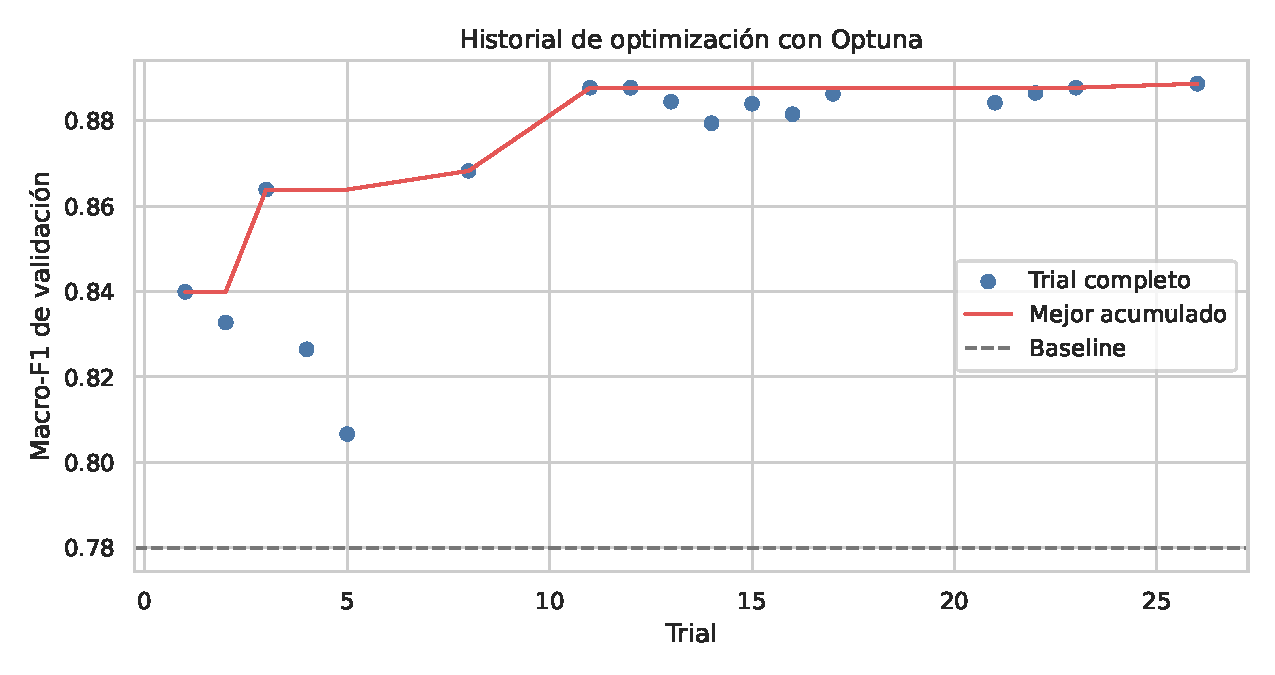
\includegraphics[width=0.88\textwidth]{optuna_history.pdf}
  \caption{Macro-F1 de los trials completos y mejor valor acumulado. La línea
  discontinua corresponde al baseline de la cabeza, no al modelo histórico.}
  \label{fig:optuna-history}
\end{figure}

\begin{figure}[H]
  \centering
  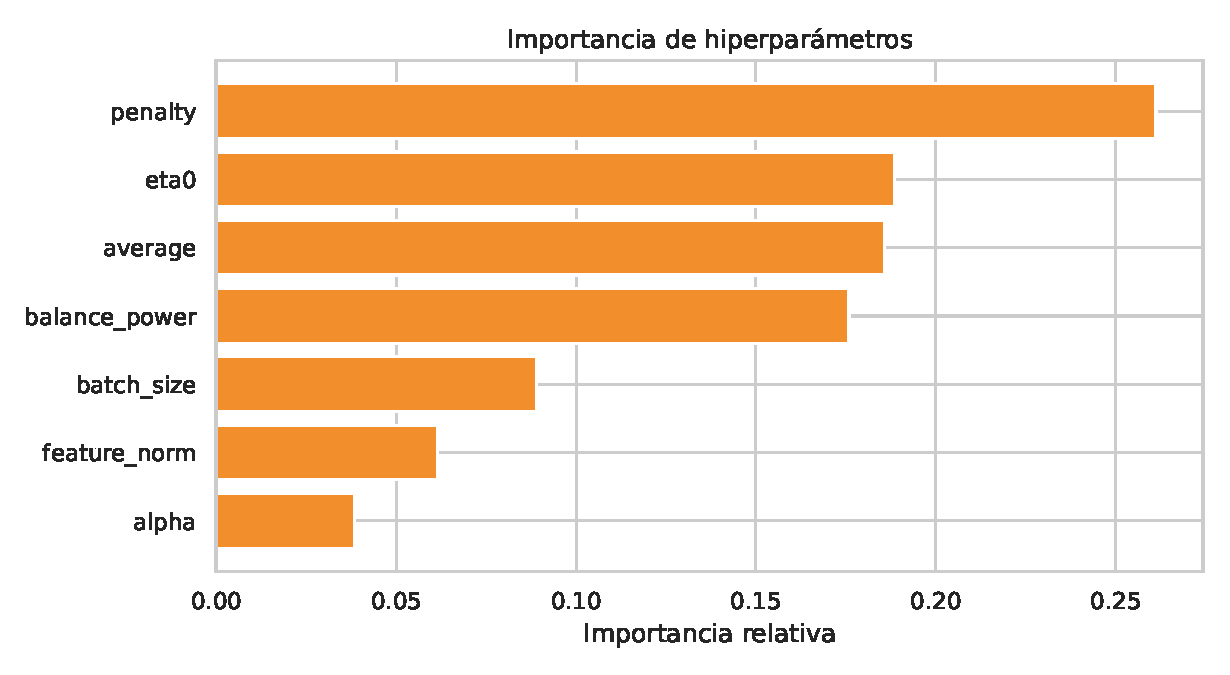
\includegraphics[width=0.86\textwidth]{optuna_importance.pdf}
  \caption{Importancia relativa calculada por Optuna dentro del espacio
  explorado. Una importancia baja no prueba que el hiperparámetro sea inútil
  fuera de esos rangos.}
  \label{fig:optuna-importance}
\end{figure}

\begin{table}[H]
  \centering
  \caption{Cinco mejores trials completos según macro-F1 de validación.}
  \label{tab:top-trials}
  \begin{tabular}{rrl}
\toprule
\textbf{Trial} & \textbf{Macro-F1 val.} & \textbf{Estado} \\
\midrule
26 & 0.8887 & COMPLETE \\
11 & 0.8877 & COMPLETE \\
12 & 0.8877 & COMPLETE \\
23 & 0.8877 & COMPLETE \\
22 & 0.8865 & COMPLETE \\
\bottomrule
\end{tabular}

\end{table}

\begin{table}[H]
  \centering
  \caption{Efecto observado del tuning sobre la misma división y backbone.}
  \label{tab:baseline-tuned}
  \begin{tabular}{lrrr}
\toprule
\textbf{Configuración} & \textbf{Accuracy} & \textbf{Macro-F1} & \textbf{F1 ponderado} \\
\midrule
baseline probe & 0.8742 & 0.7799 & 0.8685 \\
optuna tuned probe & 0.9382 & 0.8887 & 0.9383 \\
\bottomrule
\end{tabular}

\end{table}

Optuna completó 17 trials y podó 13. El mejor fue el trial 26 en la
numeración mostrada al lector (índice interno 25): penalización L2,
$\alpha=4.28\times10^{-6}$, tasa 0.000606, batch 512, potencia de balanceo
0.5, sin promedio de pesos y sin normalización L2 de embeddings. El patrón de
los mejores trials fue consistente: una regularización pequeña, tasa menor que
la del baseline y balanceo por raíz cuadrada.

El macro-F1 subió de 0.7799 a 0.8887, una ganancia absoluta de 0.1088 sobre la
misma división. Accuracy pasó de 0.8742 a 0.9382 y el cambio mayor entre los
componentes de macro-F1 apareció en recall macro: 0.7516 a 0.8914. Precision
macro también aumentó, de 0.8511 a 0.8864. El baseline no fallaba solamente por
falta de separación; estaba favoreciendo demasiado a las clases grandes. La
raíz de los pesos inversos corrigió parte de ese sesgo sin llegar al balanceo
completo, que varios trials llevaron a resultados peores.

La Figura~\ref{fig:optuna-importance} atribuye la mayor importancia a la
penalización (0.261), seguida por tasa de aprendizaje (0.189), promedio de
pesos (0.186) y potencia de balanceo (0.176). Alpha quedó en 0.038 dentro de
esta búsqueda. Esto no significa que la regularización sea irrelevante: los
trials competitivos ya se concentraron en valores pequeños. La lectura útil es
que no hizo falta aumentar la capacidad del backbone. La ganancia vino de cómo
la cabeza convirtió sus características en fronteras para clases desiguales.

\input{sections/08_modelos_avanzados}
\section{Ensemble}

\subsection{Complementariedad antes de combinar}

Un ensemble solamente puede ayudar si sus componentes aportan información
distinta. Se guardaron las nueve probabilidades de cada modelo para las 5\,015
imágenes de validación y se compararon sus conjuntos de error. Para cada pareja
se calculó la intersección y el Jaccard de errores. Un Jaccard cercano a uno
indica que ambos fallan en casi los mismos casos; un valor menor deja más margen
para que un voto corrija a uno con el otro.

Se probaron dos combinaciones. El soft voting uniforme promedió las
probabilidades de los cuatro componentes. El weighted soft voting asignó un
peso no negativo a cada uno, normalizó la suma y optimizó esos pesos con 250
trials TPE. Ni las etiquetas ni las probabilidades del holdout se usaron para
esa decisión.

\subsection{Resultado de la combinación}

\begin{table}[H]
  \centering
  \caption{Mejor componente individual frente a los dos ensembles en
  validación.}
  \label{tab:ensemble}
  \resizebox{0.94\textwidth}{!}{\begin{tabular}{lrrrrr}
\toprule
\textbf{Método} & \textbf{Accuracy} & \textbf{P-macro} & \textbf{R-macro} & \textbf{F1-macro} & \textbf{F1 pond.} \\
\midrule
EfficientNet-B0 & 0.9382 & 0.8864 & 0.8914 & 0.8887 & 0.9383 \\
uniform soft voting & 0.9535 & 0.9129 & 0.9104 & 0.9116 & 0.9535 \\
weighted soft voting & 0.9539 & 0.9209 & 0.9197 & 0.9202 & 0.9539 \\
\bottomrule
\end{tabular}
}
\end{table}

\begin{figure}[H]
  \centering
  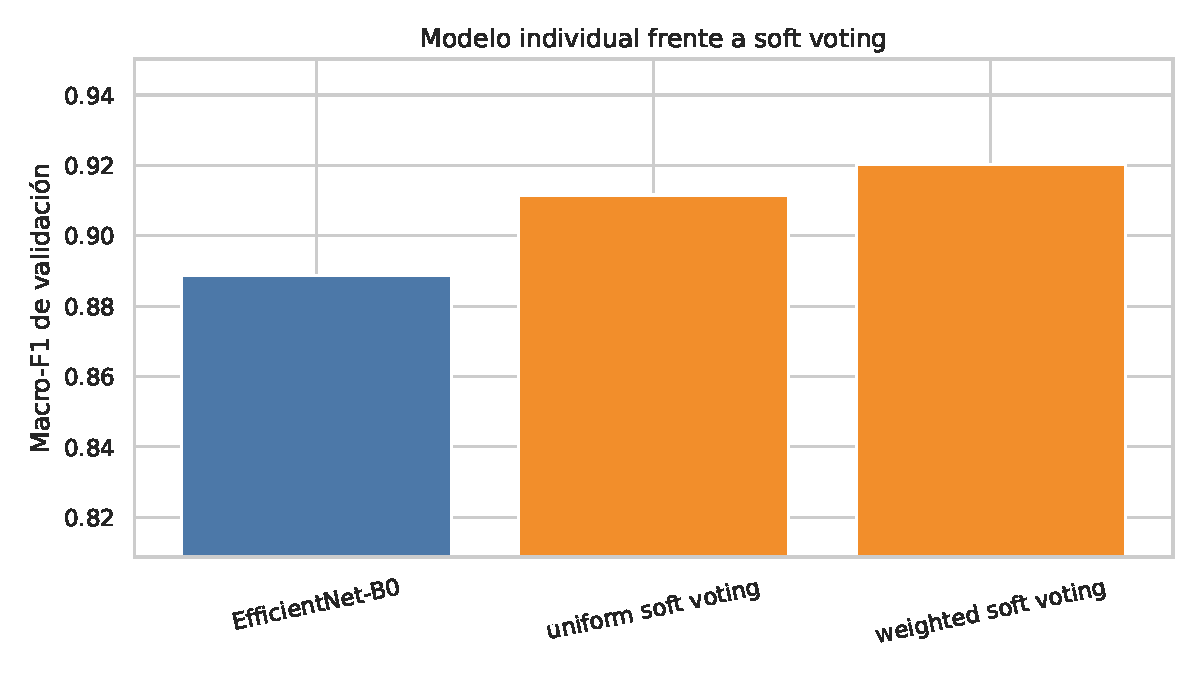
\includegraphics[width=0.82\textwidth]{ensemble_comparison.pdf}
  \caption{Cambio de macro-F1 al combinar los cuatro modelos. La escala se
  acota para que una diferencia pequeña no desaparezca visualmente.}
  \label{fig:ensemble}
\end{figure}

La regla de selección fue simple y se fijó antes del holdout: conservar el
método con mayor macro-F1 de validación, aunque fuera un modelo individual. Así
el ensemble no obtiene preferencia solamente por ser más complejo. Si la
ganancia no compensa cuatro backbones, el resultado negativo sigue siendo útil
para despliegue.

La complementariedad sí existió. EfficientNet-B0 cometió 310 errores de
validación y MobileNetV3 Small 404, pero solamente 155 fueron compartidos; su
Jaccard de errores fue 0.277, el menor de las seis parejas. B0 y ShuffleNet
compartieron 149 errores y obtuvieron Jaccard 0.281. Los modelos más débiles no
se limitaron a repetir los fallos de B0, de modo que sus probabilidades podían
corregir parte de ellos.

El promedio uniforme elevó macro-F1 de 0.8887 a 0.9116. La optimización de
pesos lo llevó a 0.9202, con 0.9539 de accuracy y 0.9197 de recall macro. Los
pesos normalizados fueron 0.3658 para EfficientNet-B0, 0.2664 para ShuffleNet,
0.2480 para MobileNetV3 y 0.1197 para FastViT. La búsqueda no eliminó los
componentes de menor F1; les asignó menos influencia porque todavía corregían
casos distintos.

La ganancia del weighted soft voting frente al mejor individuo fue 0.0315 de
macro-F1 y frente al voto uniforme 0.0086. Por esa razón pasó a validación
cruzada y holdout. El costo también se acumula: los backbones suman cerca de
38.3 MB en parámetros FP32 y aproximadamente 62.4 ms de latencia medida por
separado en esta CPU. Es la mejor selección estadística del experimento, no la
opción móvil más barata.

\section{Validación cruzada}

\subsection{Diseño}

Después de fijar hiperparámetros, arquitectura o ensemble se unieron
entrenamiento y validación en un conjunto de desarrollo de 28\,418 imágenes.
Sobre él se ejecutó StratifiedKFold de cinco partes, con barajado y semilla 42.
La estratificación utilizó la combinación clase--entorno para impedir que uno
de los folds perdiera los pocos ejemplos de roya de campo o concentrara los
fondos de laboratorio.

En cada fold la cabeza se ajustó desde cero sobre cuatro partes y se evaluó en
la quinta. Cuando la selección fue un ensemble, se reajustó una cabeza para
cada backbone y se conservaron los pesos de voting aprendidos antes. No se
volvieron a optimizar pesos dentro de los folds. Esto mide estabilidad de la
configuración fijada y evita cinco búsquedas nuevas.

\begin{table}[H]
  \centering
  \caption{Resultados de cinco folds, media y desviación estándar muestral.}
  \label{tab:cv}
  \resizebox{\textwidth}{!}{\begin{tabular}{lrrrrr}
\toprule
\textbf{Fold} & \textbf{Accuracy} & \textbf{P-macro} & \textbf{R-macro} & \textbf{F1-macro} & \textbf{F1 pond.} \\
\midrule
1 & 0.9562 & 0.9140 & 0.9144 & 0.9118 & 0.9559 \\
2 & 0.9518 & 0.9112 & 0.9080 & 0.9077 & 0.9516 \\
3 & 0.9555 & 0.9264 & 0.9160 & 0.9195 & 0.9553 \\
4 & 0.9527 & 0.9172 & 0.9123 & 0.9140 & 0.9525 \\
5 & 0.9495 & 0.9026 & 0.8923 & 0.8955 & 0.9490 \\
Media & 0.9531 & 0.9143 & 0.9086 & 0.9097 & 0.9529 \\
Desv. & 0.0027 & 0.0087 & 0.0096 & 0.0090 & 0.0028 \\
\bottomrule
\end{tabular}
}
\end{table}

\begin{figure}[H]
  \centering
  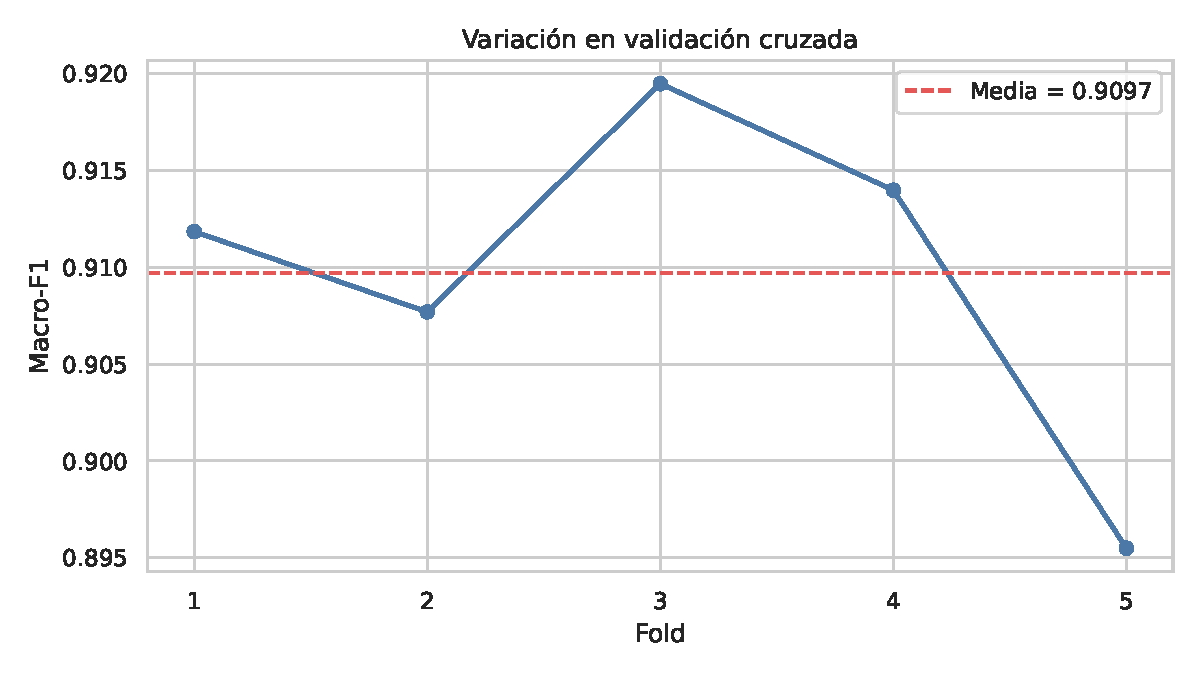
\includegraphics[width=0.82\textwidth]{cross_validation.pdf}
  \caption{Macro-F1 por fold y media de la configuración seleccionada.}
  \label{fig:cv}
\end{figure}

Esta validación no vuelve ciega la selección: Optuna y la comparación ya habían
visto una división del mismo conjunto de desarrollo. Su función es comprobar
si el resultado depende de un corte afortunado. El estimador no consultado
permanece en el holdout.

Los cinco folds produjeron 0.9097 de macro-F1 medio con desviación 0.0090. El
mejor fue el tercero (0.9195) y el menor el quinto (0.8955); la distancia entre
ambos fue 0.0240. Accuracy varió mucho menos, con media 0.9531 y desviación
0.0027. Esa diferencia entre la estabilidad de accuracy y macro-F1 vuelve a
mostrar que el movimiento ocurre en las clases pequeñas, no en el grueso del
dataset.

Potasio fue al mismo tiempo la clase con menor F1 medio (0.7039) y la más
variable (desviación 0.0496). En el quinto fold su recall cayó a 0.5524 y su F1
a 0.6304, aun cuando el accuracy global permaneció en 0.9495. Nitrógeno quedó
segundo entre los promedios bajos, con F1 0.8326, pero su desviación fue 0.0159.
Roya común y necrosis letal superaron 0.98 de F1 medio con variaciones menores
a 0.002.

La configuración es estable para las clases grandes y visualmente distintivas,
pero no para potasio. El fold bajo no invalida el ensemble; evita resumirlo como
0.91 sin decir que una partición produjo 0.63 de F1 en el problema central de
la etapa anterior. Esa variación justifica mantener métricas por clase en el
monitoreo del prototipo.

\section{Evaluación final}

\subsection{Apertura única del holdout}

Una vez fijados la configuración de la cabeza, los modelos participantes y la
regla de voting, cada cabeza se reajustó con las 28\,418 imágenes de desarrollo.
El proceso comprobó que no existiera previamente
\texttt{outputs/etapa\_2/final/metrics.json}; después creó el directorio final,
evaluó las 5\,015 filas congeladas y registró
\texttt{evaluation\_count=1}. El JSON conserva además el hash del CSV de
holdout. Esta protección no es criptográfica frente a una persona que borre
archivos, pero deja auditable la ejecución usada por el informe.

\subsection{Resultados globales y por clase}

\begin{table}[H]
  \centering
  \caption{Métricas obtenidas en la única evaluación del holdout.}
  \label{tab:final-global}
  \resizebox{0.92\textwidth}{!}{\begin{tabular}{rrrrrr}
\toprule
\textbf{Accuracy} & \textbf{P-macro} & \textbf{R-macro} & \textbf{F1-macro} & \textbf{F1 pond.} & \textbf{N} \\
\midrule
0.9537 & 0.9012 & 0.9092 & 0.9035 & 0.9537 & 5015 \\
\bottomrule
\end{tabular}
}
\end{table}

\begin{table}[H]
  \centering
  \caption{Precision, recall y F1 finales para las nueve clases.}
  \label{tab:final-class}
  \small
  \begin{tabular}{lrrrr}
\toprule
\textbf{Clase} & \textbf{Soporte} & \textbf{Precision} & \textbf{Recall} & \textbf{F1} \\
\midrule
Roya común & 338 & 0.9970 & 0.9675 & 0.9820 \\
Gusano cogollero & 729 & 0.9517 & 0.9739 & 0.9627 \\
Mancha gris & 290 & 0.9027 & 0.9276 & 0.9150 \\
Sana & 1311 & 0.9674 & 0.9748 & 0.9711 \\
Necrosis letal & 962 & 0.9927 & 0.9896 & 0.9912 \\
Def. nitrógeno & 127 & 0.7386 & 0.8898 & 0.8071 \\
Tizón norteño & 1024 & 0.9653 & 0.9248 & 0.9446 \\
Def. fósforo & 141 & 0.8553 & 0.9220 & 0.8874 \\
Def. potasio & 93 & 0.7403 & 0.6129 & 0.6706 \\
\bottomrule
\end{tabular}

\end{table}

\begin{figure}[H]
  \centering
  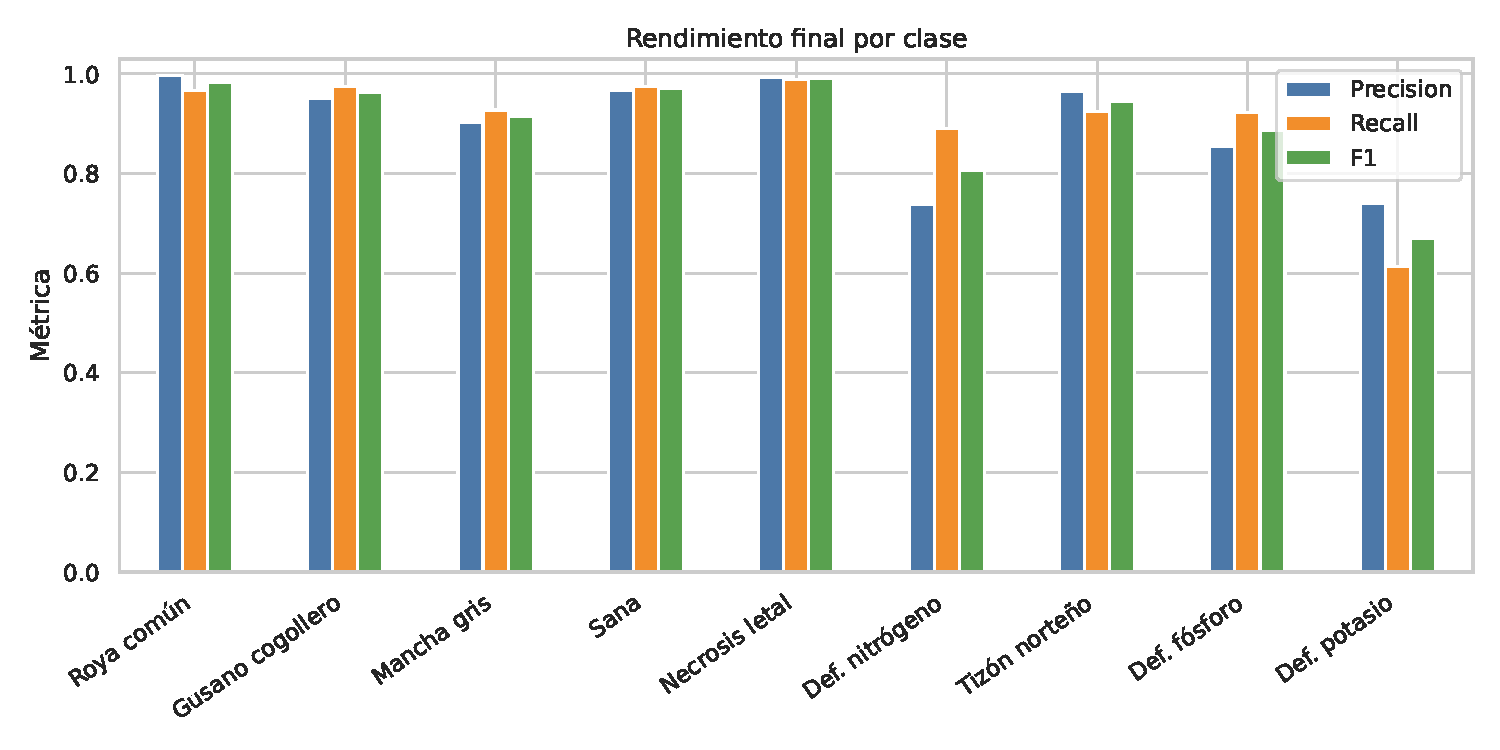
\includegraphics[width=0.90\textwidth]{final_per_class.pdf}
  \caption{Rendimiento final por clase. El soporte desigual no cambia el peso
  de cada barra en macro-F1.}
  \label{fig:final-class}
\end{figure}

El ensemble obtuvo 0.9537 de accuracy y F1 ponderado, 0.9012 de precision
macro, 0.9092 de recall macro y 0.9035 de macro-F1. El resultado quedó 0.0062
por debajo de la media de validación cruzada y dentro de una desviación
estándar de ella. La validación fija había sido más optimista (0.9202), algo
esperable porque allí también se eligieron los pesos.

La diferencia entre accuracy y macro-F1 vuelve a concentrarse en tres clases.
Necrosis letal obtuvo F1 0.9912 y roya común 0.9820; sana, gusano cogollero y
tizón norteño también superaron 0.94. Potasio quedó en 0.6706, nitrógeno en
0.8071 y fósforo en 0.8874. El ensemble mantiene el rendimiento global, pero no
convierte las deficiencias en un problema resuelto.

\subsection{Matriz de confusión}

\begin{figure}[H]
  \centering
  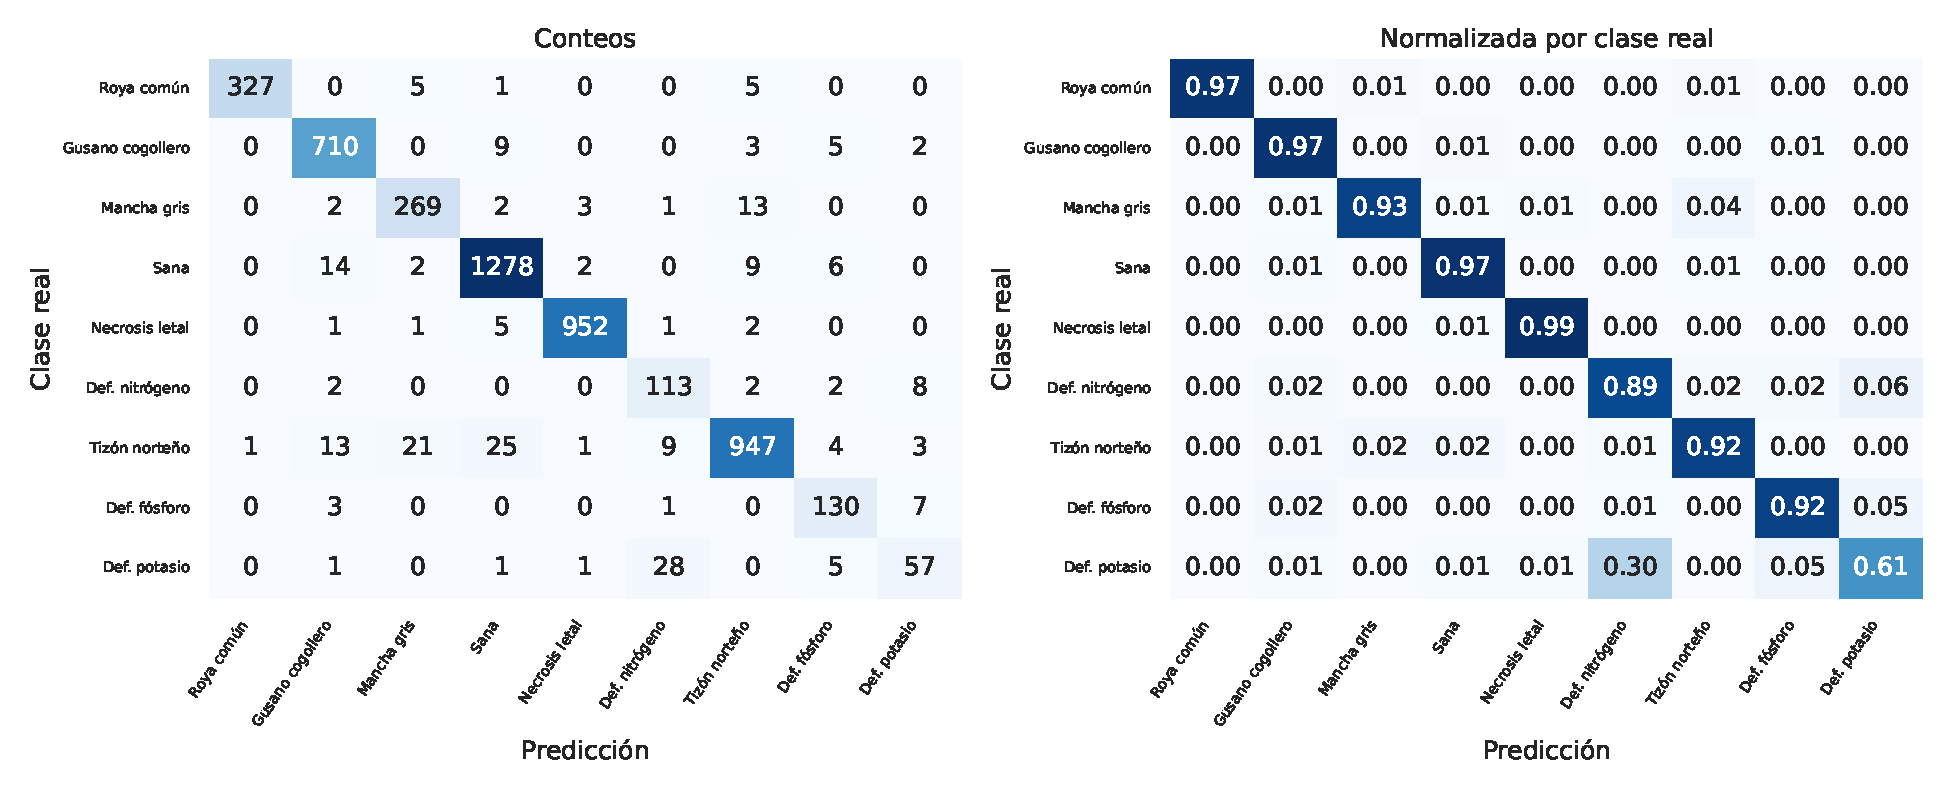
\includegraphics[width=\textwidth]{final_confusion_matrices.pdf}
  \caption{Matriz final en conteos y normalizada por clase real. La segunda
  vista permite leer clases pequeñas sin que desaparezcan detrás de la clase
  sana.}
  \label{fig:final-confusion}
\end{figure}

Hubo 232 errores en 5,015 imágenes. Los dos flujos individuales más grandes
fueron potasio hacia nitrógeno (28 casos) y tizón norteño hacia sana (25).
También aparecieron 21 casos de tizón como mancha gris y 13 en el sentido
contrario. La matriz normalizada hace visible que los 36 fallos de potasio
pesan mucho más para su clase que los 77 fallos totales de tizón para una clase
con 1,024 ejemplos.

La diagonal de roya parece casi perfecta en conteos, pero esconde una
diferencia de entorno que se revisa en fairness: 327 de 338 casos fueron
correctos y los once errores se concentran proporcionalmente en las pocas
imágenes de campo. El problema no está en reconocer el patrón de laboratorio,
sino en sostenerlo cuando cambia la captura.

\subsection{Etapa 1 frente a Etapa 2}

\begin{table}[H]
  \centering
  \caption{Referencias de ambas etapas. Accuracy y macro-F1 no son una
  comparación controlada porque cambiaron corpus, división y entrenamiento.}
  \label{tab:e1-e2}
  \resizebox{\textwidth}{!}{\begin{tabular}{lrrl}
\toprule
\textbf{Métrica} & \textbf{Etapa 1} & \textbf{Etapa 2} & \textbf{Lectura} \\
\midrule
Accuracy & 0.9521 & 0.9537 & Corpus y protocolo distintos \\
Macro-F1 & 0.9146 & 0.9035 & Corpus y protocolo distintos \\
Recall potasio & -- & 0.6129 & No comparable \\
F1 potasio & 0.62 & 0.6706 & Referencia B0 histórica \\
Imágenes potasio & 266 & 621 & +355 \\
\bottomrule
\end{tabular}
}
\end{table}

La tabla no atribuye el cambio a Optuna ni a la ampliación. El contraste
controlado de tuning está en la Tabla~\ref{tab:baseline-tuned}; aquí la Etapa 1
aporta el antecedente del proyecto y la Etapa 2 aporta un holdout que sí
permaneció cerrado. Esta diferencia metodológica vale más que aparentar una
ganancia directa entre dos números obtenidos bajo condiciones distintas.

Como referencia, accuracy cambió de 0.9521 a 0.9537 y macro-F1 de 0.9146 a
0.9035. No se interpreta la caída de 0.0111 como empeoramiento causal: el
holdout nuevo contiene otro corpus y la cabeza no fue ajustada end-to-end. En
potasio, el F1 pasó de 0.62 a 0.6706 y el soporte evaluado de 40 a 93. La señal
es favorable, pero todavía insuficiente y tampoco aislable de los cambios de
datos y protocolo.

\input{sections/12_analisis_errores}
\section{Interpretabilidad}

La Etapa 1 ya explicó LIME y Grad-CAM; aquí se aplicaron al modelo final en vez
de repetir su teoría. Se seleccionaron cinco situaciones desde el CSV del
holdout: acierto fácil, acierto difícil, error de alta confianza, deficiencia
nutricional de potasio y una imagen de laboratorio con fondo controlado. La
selección fue programática y el archivo \texttt{cases.csv} conserva ruta,
etiqueta, predicción, confianza, entorno y fuente.

Cuando el método final fue un ensemble, se calculó Grad-CAM para la clase
predicha en la última capa convolucional de cada componente. Cada mapa se
normalizó y se combinó con los mismos pesos del soft voting. La visualización
localiza regiones que influyeron en los componentes, pero sigue siendo una
aproximación de la decisión conjunta. Grad-CAM no prueba que la región sea una
causa biológica \citep{selvaraju2017gradcam}.

\begin{figure}[H]
  \centering
  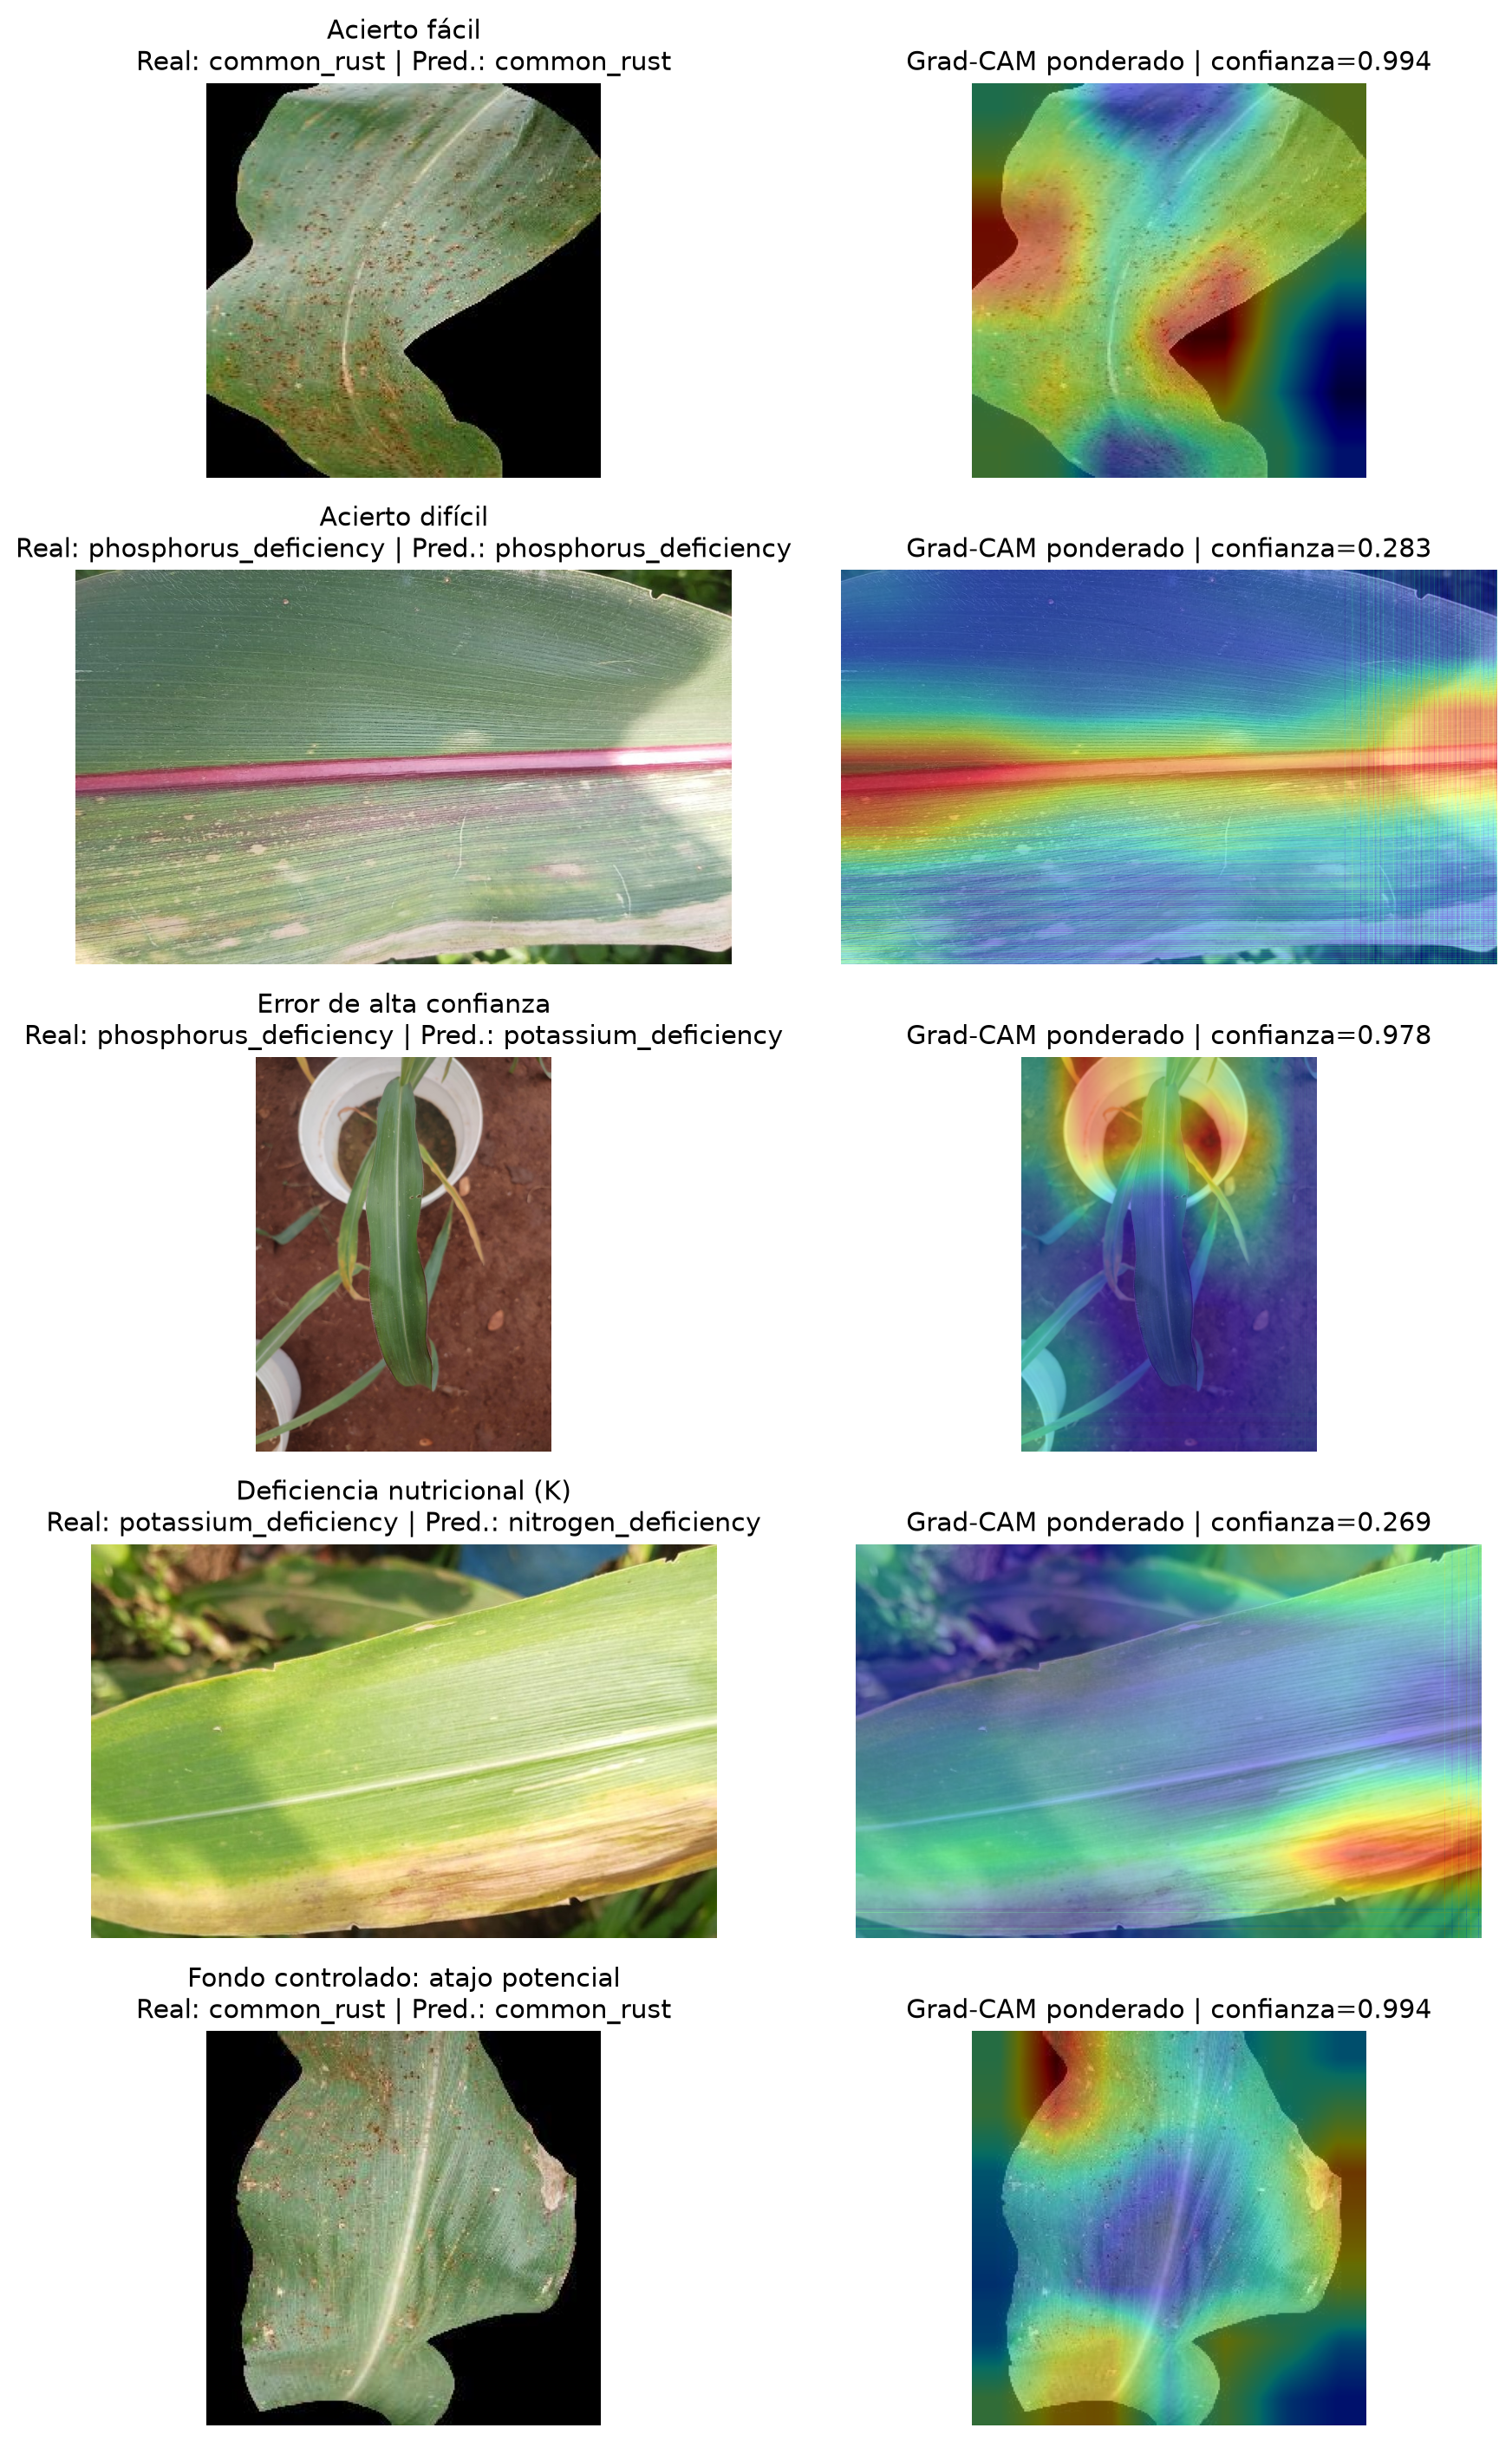
\includegraphics[height=0.82\textheight,keepaspectratio]{final_gradcam_cases.png}
  \caption{Casos del holdout y mapas Grad-CAM del método final. El color rojo
  marca mayor activación relativa dentro de cada imagen.}
  \label{fig:gradcam-final}
\end{figure}

El acierto difícil de fósforo tuvo solamente 0.283 de confianza y concentró la
activación sobre la nervadura con coloración púrpura. El modelo miró una señal
coherente y aun así dejó probabilidades cercanas para otras clases. En el caso
de potasio predicho como nitrógeno (0.269), el mapa cayó sobre el borde
amarillento y necrótico. Aquí el modelo mira el lugar correcto y aun así se
equivoca: el problema está en separar dos patrones nutricionales, no en haber
ignorado la hoja.

El error de mayor confianza cuenta otra historia. La imagen de fósforo
clasificada como potasio con 0.978 activa con fuerza el borde de la maceta y el
suelo alrededor, mientras buena parte de la hoja queda fría. Ese caso combina
fondo, encuadre vertical y amarillamiento, y muestra un atajo más preocupante
que una frontera fina entre lesiones. Los dos aciertos de roya sobre fondo
negro también producen zonas calientes cerca del contorno recortado. La red
usa puntos de roya, pero el borde artificial participa en la decisión.

LIME se ejecutó sobre el error de alta confianza cuando existió uno; de lo
contrario, sobre el acierto difícil. Se usaron 32 perturbaciones y ocho
superpíxeles visibles sobre EfficientNet-B0, el componente con mayor peso del
ensemble. A diferencia de Grad-CAM, LIME pregunta cómo cambia la salida al
ocultar segmentos de esa imagen \citep{ribeiro2016why}. Con tan pocas
perturbaciones se busca una comprobación cualitativa reproducible, no una
estimación estable para todas las hojas ni una explicación del voto completo.
La copia usada por LIME limita su lado mayor a 512 píxeles antes de generar
perturbaciones; el clasificador de todas formas la reduce a 224.

\begin{figure}[H]
  \centering
  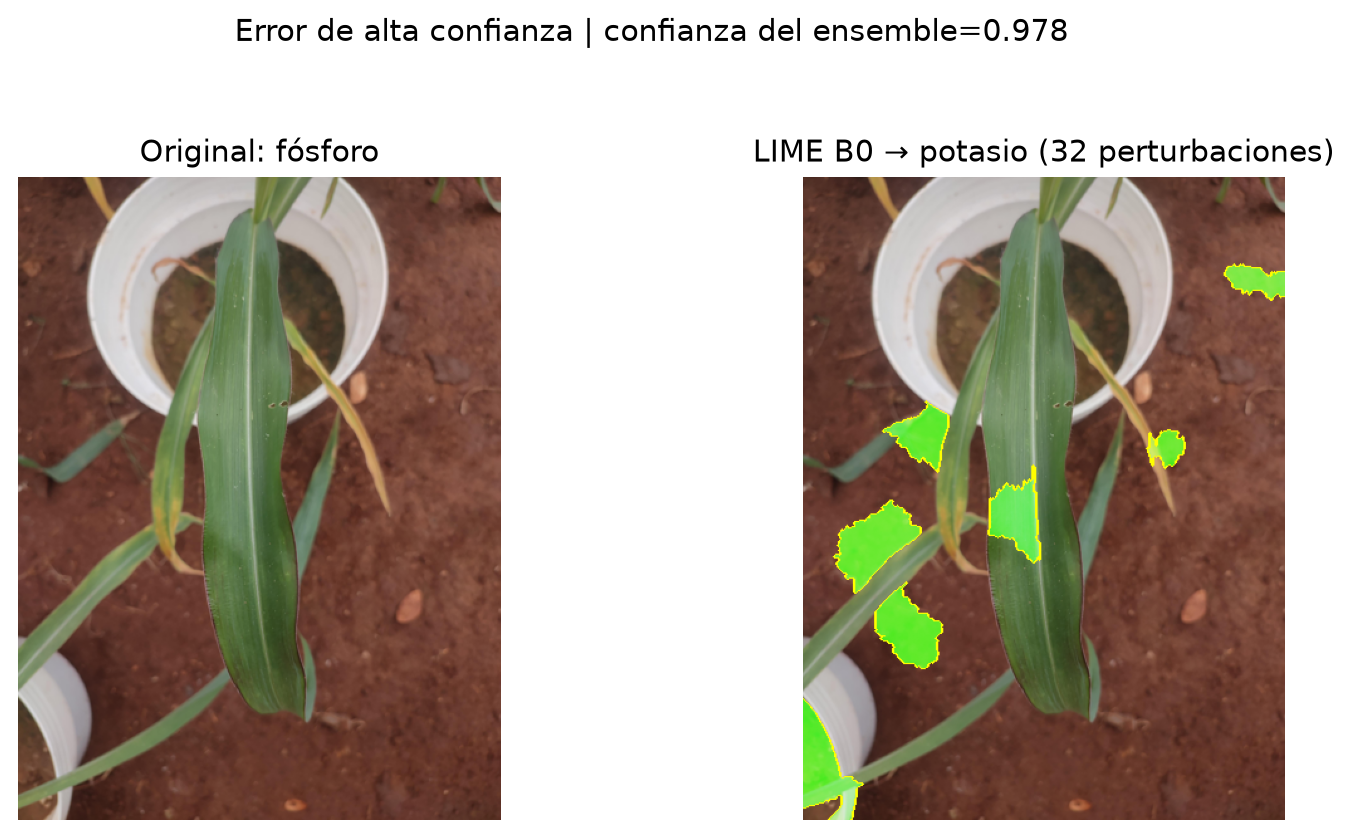
\includegraphics[width=0.90\textwidth]{final_lime_case.png}
  \caption{Imagen final seleccionada y explicación local LIME. Los bordes
  corresponden a segmentos perturbados, no a una segmentación agronómica de la
  lesión.}
  \label{fig:lime-final}
\end{figure}

La explicación LIME se aplicó al mismo error fósforo--potasio de 0.978. Los
segmentos influyentes no quedaron encerrados en la hoja central: aparecen sobre
un fragmento de su tejido, hojas vecinas, suelo y el borde de otra maceta. Junto
con el Grad-CAM concentrado alrededor de la maceta superior, ambos métodos
indican que la salida mezcla una señal foliar débil con el contexto de captura.
La figura no se usa para corregir la etiqueta. Sirve para decidir qué tipo de
ejemplo debe añadirse: hojas con síntomas semejantes, pero fondos y encuadres
diferentes.

SHAP existe en la infraestructura histórica del repositorio, pero no se ejecutó
sobre la cabeza final. Por esa razón no se incluye una figura SHAP reciclada
como si perteneciera a esta corrida. La evidencia final de interpretabilidad
son los mapas y metadatos generados por los dos métodos anteriores.

\input{sections/13_fairness}
\section{Consideraciones éticas}

El riesgo principal de Doctor Maíz no es que una métrica baje unas décimas,
sino que una persona convierta una predicción en una acción sobre el cultivo.
Un falso negativo puede retrasar la consulta cuando la planta presenta necrosis
letal o tizón. Un falso positivo de deficiencia puede inducir una aplicación de
fertilizante que no era necesaria. También puede existir una predicción
visualmente razonable pero agronómicamente incompleta: síntomas parecidos
pueden tener causas distintas y una fotografía no contiene información sobre
suelo, clima, etapa fenológica o evolución temporal.

\subsection{Confianza y comunicación del resultado}

La interfaz no presenta el resultado como un diagnóstico confirmado. Muestra
probabilidad, segunda clase cuando la confianza es menor de 0.70 y un mensaje
específico cuando el detector fuera de dominio rechaza la imagen. La demo
experimental emplea un umbral de 0.60 para advertir baja confianza y acompaña
cada salida con la frase «Apoyo orientativo; no sustituye la evaluación de un
profesional agrónomo». Estos umbrales son controles de interfaz, no garantías
estadísticas. No se ejecutó una calibración formal sobre el holdout y, por
tanto, 80\% de confianza no debe leerse como 80\% de certeza clínica o
agronómica.

El rechazo fuera de dominio de la aplicación usa distancia relativa de
Mahalanobis sobre un segundo tensor de características. Además, rechaza
distribuciones con poca separación. Esto reduce el riesgo de clasificar una
persona, una herramienta o una hoja de otra especie como una de las nueve
clases. No cubre todas las imágenes extrañas posibles y pertenece al modelo
móvil histórico, no al ensemble experimental. La selección de Etapa 2 todavía
no incorpora su propio detector OOD.

\subsection{Errores con costos distintos}

Las nueve clases no tienen el mismo costo de error. Confundir nitrógeno con
potasio puede terminar en una recomendación de manejo distinta; confundir una
hoja sana con una enfermedad puede causar gasto y preocupación; declarar sana
una hoja enferma puede demorar atención. El entrenamiento optimiza macro-F1,
que protege estadísticamente a las clases pequeñas, pero no incorpora una matriz
de costos agronómicos. Esa matriz debe definirse con especialistas y con
información de manejo local antes de convertir el modelo en un sistema de
decisión.

Por esa razón las recomendaciones de la app deben entenderse como pasos de
inspección: revisar otras hojas, observar la distribución del síntoma, repetir
la captura y consultar asistencia técnica. No corresponde indicar dosis o
productos solamente a partir del logit más alto. Una recomendación automática
de insumos sería una función nueva, con riesgos y validación distintos a los de
clasificar una imagen.

\subsection{Datos, ubicación y trazabilidad}

La base móvil almacena localmente ruta de imagen, etiqueta, confianza,
distribución y fecha. También reserva campos opcionales de latitud y longitud.
La operación offline evita enviar cada fotografía por defecto, pero no elimina
el riesgo de privacidad si más adelante se sincroniza una contribución. La
ubicación de una parcela puede revelar domicilio, patrón productivo o actividad
económica. Debe solicitarse consentimiento separado, explicar el propósito,
reducir precisión cuando no sea necesaria y permitir borrar el dato.

Cada predicción que se use para seguimiento debería conservar versión del
modelo, hash del artefacto, fecha y origen del resultado. La aplicación
inspeccionada valida el orden de etiquetas y el contrato de tensores; el
manifiesto del modelo registra arquitectura y SHA-256. Esa trazabilidad evita
un problema concreto: que una corrección del usuario quede asociada a un modelo
distinto del que produjo el diagnóstico.

\subsection{Supervisión y salida segura}

El sistema debe permitir «no sé». Una foto desenfocada, una hoja pequeña dentro
del encuadre o una condición que no pertenece a las nueve clases necesita
terminar en repetición de captura o consulta, no en una recomendación forzada.
El protocolo de campo propuesto incluye revisar varios órganos de la planta y
no actuar sobre una sola imagen. Las correcciones guardadas por productores o
extensionistas tampoco deben incorporarse automáticamente al entrenamiento:
primero requieren revisión agronómica, control de duplicados y registro de
procedencia.

Estas medidas no convierten el sistema en inocuo. Hacen visible dónde termina
la clasificación y dónde empieza una decisión humana. Ese límite es
especialmente necesario porque las métricas finales provienen de colecciones
públicas y no de una validación prospectiva en parcelas salvadoreñas.

\section{Prototipo funcional}

\subsection{Arquitectura verificada}

La evidencia operativa combina dos piezas. La primera es la demo reproducible
de esta etapa, que ejecuta la selección final sobre una imagen real. La segunda
es la aplicación móvil Doctor Maíz inspeccionada en el commit
\nolinkurl{dd048d37dcabd08c53c704d702825e7d672f0f37}. La aplicación usa React
Native 0.86, Expo 57, TypeScript, WatermelonDB y
\texttt{react-native-fast-tflite}. El modelo embarcado es
EfficientNet-Lite0 TFLite con pesos int8, entrada y salida float32 y tamaño de
3\,743\,824 bytes. Su SHA-256 coincide con el manifiesto:
\par\smallskip\noindent
\texttt{3a0623cd985a23b954e424e605a2e00c}\allowbreak
\texttt{91f8d592e376dfe3149e5820485bc2b3}.

\begin{figure}[H]
  \centering
  \fbox{\begin{minipage}{0.88\textwidth}
    \centering
    \textbf{Cámara o galería}
    $\longrightarrow$ orientación EXIF, RGB y $224\times224$
    $\longrightarrow$ \textbf{TFLite local}\\[0.3em]
    $\longrightarrow$ logits + características OOD
    $\longrightarrow$ Top-1, confianza y rechazo
    $\longrightarrow$ \textbf{resultado e historial offline}
  \end{minipage}}
  \caption{Flujo real implementado en la aplicación móvil. La API participa en
  autenticación, sincronización y actualización; la inferencia ocurre en el
  dispositivo.}
  \label{fig:prototype-flow}
\end{figure}

El motor materializa el modelo como archivo local, comprueba que el tensor de
entrada tenga $1\times3\times224\times224$ elementos y que existan nueve
salidas en el orden de \texttt{labels.json}. También exige un segundo tensor de
características para el detector OOD. La pantalla de captura acepta cámara o
galería, ejecuta preprocesamiento e inferencia, navega al resultado y guarda el
escaneo. La pantalla siguiente muestra la fotografía, diagnóstico, confianza,
segunda opción en casos de confianza baja y recomendaciones. Si la imagen se
rechaza, no fuerza una enfermedad: pide acercarse a una hoja con mejor luz.

\subsection{Comprobación ejecutable}

Se instaló el lockfile del repositorio móvil en un clon temporal. La instalación
normal detectó un conflicto entre React Native 0.86.0 y
\texttt{@react-native/jest-preset} 0.86.2; se completó con
\texttt{npm ci --legacy-peer-deps}. Después, \texttt{npm run typecheck} terminó
sin errores y \texttt{npm test -- --runInBand} aprobó 40 suites y 276 pruebas.
Las advertencias de React sobre \texttt{act(...)} no cambiaron el código de
salida. El entorno disponible usa Node 18.19.1 aunque dependencias recientes
solicitan Node 20.19.4 o superior; reproducir la app requiere alinear esa
versión. La instalación también reportó 24 vulnerabilidades de dependencias
(17 moderadas y 7 altas). No se ejecutó una actualización forzada porque
habría cambiado el lockfile del prototipo; deben revisarse antes de distribuir
otra compilación.

La Figura~\ref{fig:prototype-capture} es una captura generada por ejecución, no
una maqueta. El comando carga los pesos públicos del o de los backbones
seleccionados, aplica la cabeza final y escribe un JSON con Top-3, confianza y
latencia CPU. Se usa una imagen del holdout solo después de terminar la
evaluación final.

\begin{figure}[H]
  \centering
  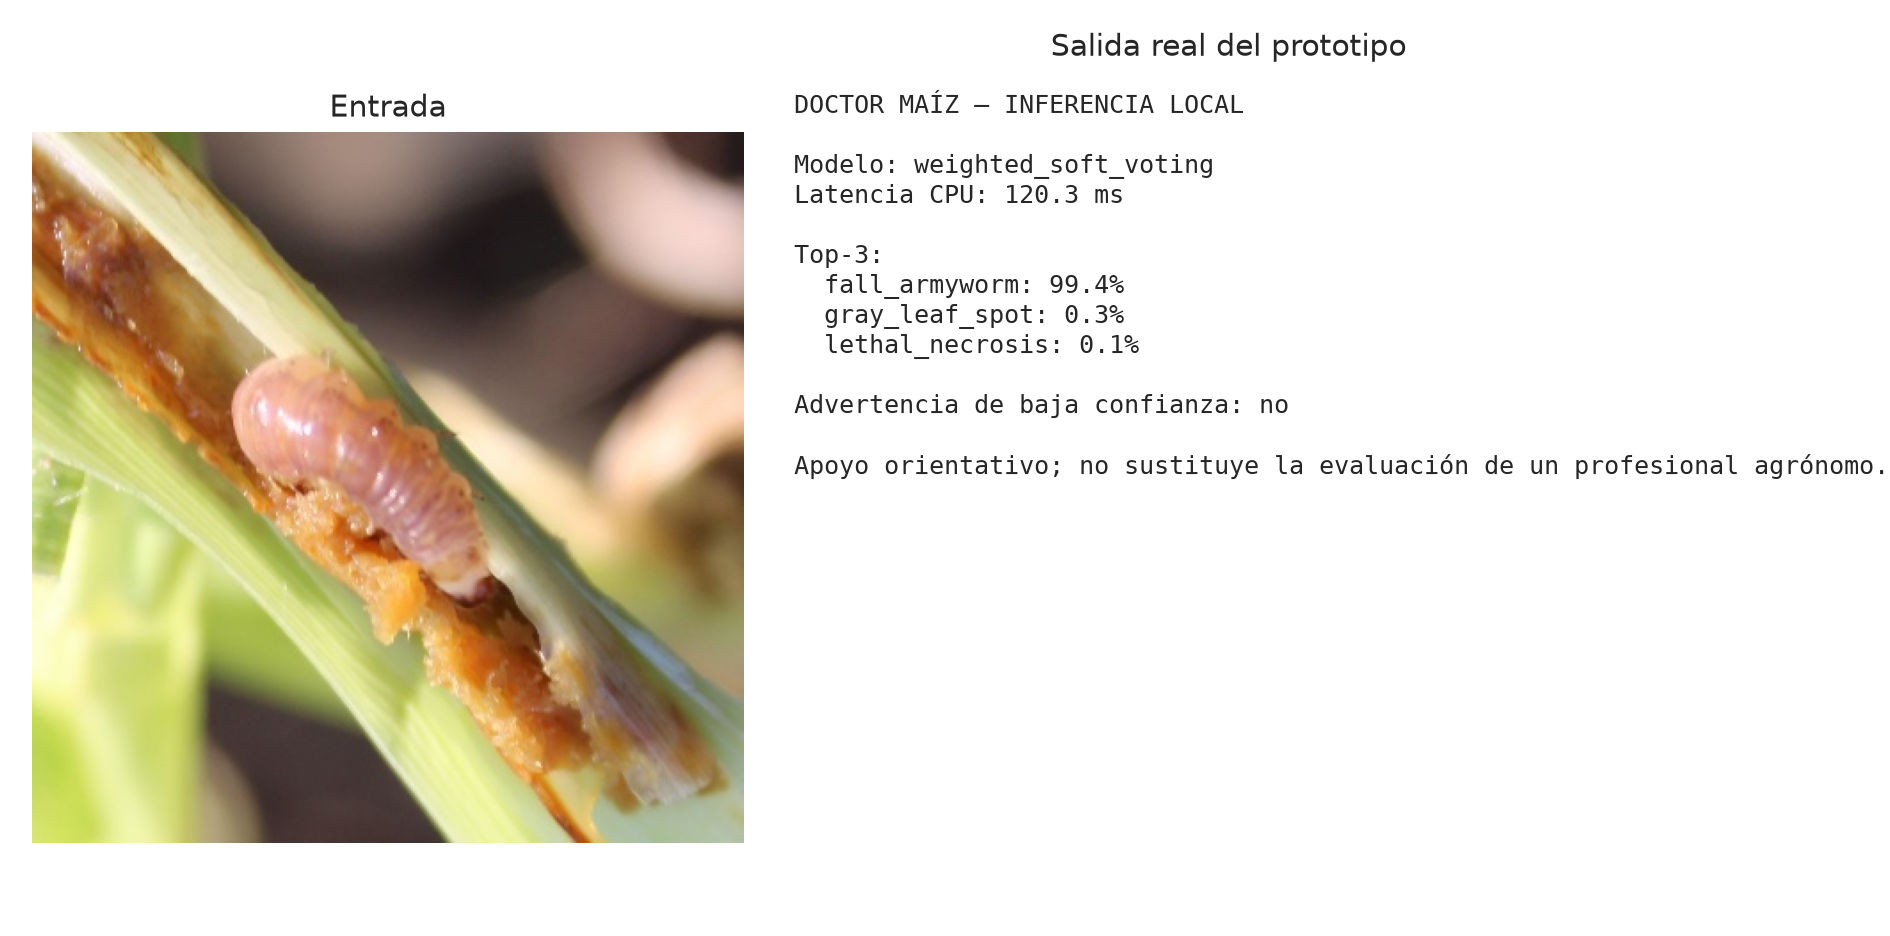
\includegraphics[width=0.94\textwidth]{prototype_capture.png}
  \caption{Captura de la demo de Etapa 2: entrada real y salida producida por el
  pipeline final. La latencia corresponde a CPU de escritorio y no se presenta
  como benchmark Android.}
  \label{fig:prototype-capture}
\end{figure}

La demo se reproduce desde la raíz del clasificador con:

\begin{verbatim}
PYTHONPATH=.:/tmp/doctor-maiz-pydeps python \
  scripts/etapa_2/stage2_experiments.py \
  --output-dir outputs/etapa_2 demo --image /ruta/hoja.jpg
\end{verbatim}

\subsection{Qué modelo está desplegado}

La aplicación móvil conserva EfficientNet-Lite0 de la línea de entrenamiento
principal, no la cabeza congelada evaluada en esta etapa. Hacer el reemplazo
habría requerido exportar conjuntamente backbone, escalado y regresión
one-vs-rest, validar paridad y volver a medir OOD en Android. Ninguna de esas
pruebas se ejecutó, así que el informe no afirma un despliegue que no ocurrió.
El prototipo demuestra que la arquitectura de integración existe y que el
artefacto histórico funciona dentro de ella; la demo demuestra que la selección
experimental produce resultados reproducibles.

Durante una primera consulta, el endpoint de salud respondió
\texttt{\{"status":"ok"\}} y el endpoint de versión informó Android 1.0.0,
código 6. En la verificación final del mismo día, el dominio dejó de resolver
por DNS y la URL de APK sin autenticación devolvió HTTP 404. Por eso el
prototipo se califica como funcional e integrado, pero no como un despliegue
público con disponibilidad comprobada de extremo a extremo. Esta diferencia
reduce la puntuación del criterio y queda como limitación operativa, no como
pendiente oculto.

\section{Impacto social}

\subsection{Una herramienta de primera observación}

Para un pequeño productor, el valor posible de Doctor Maíz no está en reemplazar
un laboratorio ni en emitir una receta. Está en reducir la distancia entre
notar un síntoma y formular una pregunta útil. Una foto puede sugerir si el
patrón se parece más a roya, tizón, daño de gusano cogollero o una deficiencia,
mostrar alternativas y conservar un registro para enseñarlo a un extensionista.
La detección temprana solo ocurre si la captura se hace cuando el síntoma es
visible y si la respuesta conduce a una revisión posterior.

La operación local cambia la viabilidad en zonas con conexión irregular. El
modelo móvil no necesita enviar la fotografía para inferir y WatermelonDB
conserva historial y correcciones hasta que exista conectividad. Esto reduce
consumo de datos y permite trabajar en una parcela sin señal. También concentra
el costo en el teléfono: cámara, memoria y tiempo de inferencia deben ser
aceptables en dispositivos de gama baja, algo que todavía no se midió con una
muestra representativa de equipos.

\subsection{Productores y extensionistas}

Usado individualmente, el sistema puede ayudar a organizar observaciones:
fotografiar varias hojas, comparar confianza, anotar una corrección y decidir
si hace falta asistencia. Usado por extensionistas, puede funcionar como una
ficha común para priorizar visitas y recopilar ejemplos difíciles. El segundo
uso parece más seguro porque una persona con experiencia interpreta el
resultado junto con etapa del cultivo, distribución del daño y condiciones del
suelo.

La cobertura de nueve clases limita ambas funciones. El maíz puede presentar
otras enfermedades, daños por herbicida, sequía, plagas o síntomas combinados.
Una categoría ausente no se convierte en visible por tener un detector OOD.
El usuario necesita una salida clara para «ninguna de las anteriores» y una
ruta de consulta. De lo contrario, la facilidad de tomar una foto puede
producir más confianza de la que permite el dataset.

\subsection{Beneficio posible y evidencia disponible}

El proyecto no midió aumento de rendimiento, ahorro de fertilizante, reducción
de pérdidas ni tiempo de respuesta de asistencia técnica. Atribuirle cualquiera
de esos porcentajes sería inventar impacto. Lo que sí se comprobó es una cadena
técnica: clasificación sobre un corpus amplio, evaluación separada, análisis
por condiciones, inferencia local y mecanismo de corrección. Esa cadena hace
posible una prueba de campo; todavía no demuestra un beneficio agronómico.

Una evaluación de impacto debería comparar prácticas, no solamente modelos.
Por ejemplo, se pueden asignar comunidades o extensionistas a tres condiciones:
procedimiento habitual, acceso a Doctor Maíz y acceso a Doctor Maíz con revisión
técnica. Las medidas relevantes serían tiempo hasta la consulta, concordancia
con diagnóstico agronómico, decisiones evitadas por baja confianza y tasa de
seguimiento. Rendimiento e insumos solo deberían medirse con un diseño que
controle clima, variedad y manejo.

\subsection{Riesgos de exclusión}

El lenguaje, la alfabetización digital y el diseño del teléfono influyen tanto
como el clasificador. Mostrar nombres en inglés, cifras sin explicación o
pantallas cargadas puede excluir a la población a la que se busca apoyar. La
aplicación ya presenta etiquetas y recomendaciones en español, pero no se
realizó una prueba de usabilidad con productores. Tampoco se evaluaron
variantes lingüísticas, accesibilidad visual o instrucciones por audio.

El dataset introduce otra exclusión: proviene de colecciones externas y no
identifica municipios salvadoreños. Un macro-F1 alto puede convivir con fallos
en una variedad local, una cámara económica o una iluminación no representada.
Por eso el despliegue responsable empieza pequeño, registra contexto con
consentimiento y permite detener el uso si una región muestra una brecha
persistente.

\subsection{Condiciones para uso real}

Antes de promover el sistema a escala se necesitan, como mínimo: validación
prospectiva en parcelas; revisión de etiquetas por profesionales; protocolo de
captura sencillo; prueba en teléfonos de distintas gamas; monitoreo por región
y clase; canal de corrección; política de datos y ubicación; y un responsable
que revise incidentes. Bajo esas condiciones, Doctor Maíz puede ampliar el
alcance de la asistencia. Sin ellas, solo traslada al teléfono la incertidumbre
del dataset.

\section{Recomendaciones de política pública}

Las siguientes medidas son propuestas derivadas del experimento. No se
presentan como programas vigentes ni como decisiones ya adoptadas.

\begin{enumerate}
  \item \textbf{Crear un conjunto nacional con procedencia verificable.}
  Instituciones académicas, asociaciones de productores y servicios de
  extensión pueden acordar un esquema común para fotografías de hojas, con
  municipio a una resolución apropiada, variedad, etapa fenológica, fecha,
  dispositivo y diagnóstico de referencia. La diversidad regional debe
  medirse, no asumirse.

  \item \textbf{Estandarizar la captura sin volverla artificial.}
  Cada registro debería incluir una vista cercana del síntoma y otra de la
  planta, bajo luz disponible, además de una guía de enfoque. El protocolo
  necesita ejemplos reales de fondos complejos; llenar el dataset de fondos
  blancos mejoraría el laboratorio y empeoraría la pregunta de campo.

  \item \textbf{Establecer revisión agronómica de etiquetas.}
  Una corrección enviada desde la app no debe convertirse directamente en
  ground truth. Se requiere doble revisión para casos dudosos, registro del
  criterio usado y una categoría de desacuerdo. Las deficiencias N/P/K merecen
  prioridad porque su similitud visual fue el principal problema de ambas
  etapas.

  \item \textbf{Usar el sistema como apoyo de extensión.}
  El primer despliegue debería entregar la herramienta a equipos técnicos y a
  grupos acompañados de productores. Esto permite contrastar la predicción con
  síntomas de la parcela, corregir recomendaciones y definir cuándo la app debe
  derivar a una visita.

  \item \textbf{Monitorear por región, clase y dispositivo.}
  Accuracy global no basta. Un tablero de operación debe seguir recall de
  clases críticas, tasa de rechazo, correcciones, latencia y brechas entre
  cámaras o zonas. Los grupos con soporte pequeño deben mostrarse con su
  incertidumbre y no ocultarse bajo promedios nacionales.

  \item \textbf{Minimizar y proteger ubicación.}
  La georreferencia debe ser opcional, separada del uso básico y explicada en
  lenguaje claro. Cuando el objetivo sea vigilancia regional, puede
  almacenarse una cuadrícula o municipio en vez de coordenadas exactas. Deben
  definirse retención, acceso, eliminación y respuesta ante filtraciones.

  \item \textbf{Financiar el ciclo de retroalimentación.}
  Recoger casos difíciles sin personal que los revise crea una cola, no un
  dataset. El presupuesto debe incluir validación, curación, deduplicación,
  versionado y reentrenamiento, además del desarrollo de la aplicación.

  \item \textbf{Exigir validación de campo antes del uso masivo.}
  Una versión candidata debe aprobar criterios predefinidos de rendimiento por
  clase y entorno, prueba de teléfonos, estabilidad offline y comprensión del
  mensaje de incertidumbre. Una caída grande en potasio o en una región debe
  detener la promoción aunque el accuracy global siga alto.

  \item \textbf{Publicar una ficha de cada versión.}
  La ficha debe incluir corpus, fingerprint, clases, protocolo, métricas por
  grupo, limitaciones, hash del modelo y cambios desde la versión anterior,
  siguiendo la idea de reportes de modelo \citep{mitchell2019modelcards}.
  Esto permite saber qué produjo un diagnóstico meses después.
\end{enumerate}

Estas recomendaciones colocan el mayor esfuerzo donde el experimento encontró
la mayor fragilidad: datos con contexto, revisión y seguimiento. Comprar más
capacidad de cómputo puede facilitar el entrenamiento, pero no resuelve una
etiqueta ambigua ni una región ausente. La política útil conecta el modelo con
una red de asistencia y con reglas para corregirlo.

\section{Limitaciones}

\begin{enumerate}
  \item \textbf{No hubo ajuste fino end-to-end en la corrida nueva.} La máquina
  disponible no expuso CUDA. Se compararon backbones ImageNet congelados con
  una cabeza logística optimizada. Es un experimento completo sobre el corpus,
  pero no demuestra el rendimiento que tendrían las mismas arquitecturas al
  adaptar todos sus pesos.

  \item \textbf{La comparación con Etapa 1 no es controlada.} Cambiaron corpus,
  división, objetivo de entrenamiento y familia de cabeza. Las diferencias
  históricas ayudan a entender el proyecto; no aíslan el efecto causal de la
  ampliación o de Optuna.

  \item \textbf{Los grupos de entorno están confundidos con la clase.}
  Solamente roya, mancha gris y tizón norteño tienen imágenes tanto de
  laboratorio como de campo. El gap global resume el dataset, no mide por sí
  solo el efecto de retirar un fondo uniforme.

  \item \textbf{Faltan metadatos de campo.} No se conoce finca, municipio,
  variedad, teléfono, campaña o evaluador. La fuente del archivo no reemplaza
  esos datos y puede estar asociada simultáneamente con clase, resolución y
  estilo de captura.

  \item \textbf{Blur y resolución son indicadores indirectos.} La varianza del
  Laplaciano depende del contenido de la lesión y la compresión, no solamente
  del enfoque. Los terciles describen diferencias internas y no fijan un
  umbral universal de calidad.

  \item \textbf{La validación cruzada es condicional a una selección previa.}
  Arquitectura, hiperparámetros y ensemble se eligieron con la división
  train/validación. Los cinco folds posteriores miden estabilidad dentro del
  desarrollo; el estimador verdaderamente no consultado es el holdout final.

  \item \textbf{No se calibraron probabilidades.} La confianza sirve para
  ordenar alternativas y activar una advertencia de interfaz, pero no se
  comprobó confiabilidad mediante ECE, diagrama de calibración o temperatura
  ajustada en un conjunto separado.

  \item \textbf{La explicación del ensemble es aproximada.} Grad-CAM combina
  mapas normalizados de componentes usando los pesos de soft voting. Esto ayuda
  a localizar regiones influyentes, pero no produce una descomposición causal
  exacta de la probabilidad conjunta. LIME usa 32 perturbaciones en un caso y
  explica solo EfficientNet-B0, el componente de mayor peso.

  \item \textbf{La latencia no es móvil.} Los valores comparativos de backbones
  y la demo corresponden a CPU de escritorio. El artefacto móvil histórico sí
  está integrado, pero no se ejecutó un benchmark en varios teléfonos Android
  durante esta etapa.

  \item \textbf{Disponibilidad pública no confirmada al cierre.} La aplicación
  aprobó typecheck y 276 pruebas, pero el dominio de la API dejó de resolver en
  la comprobación final y la URL de APK respondió 404 sin autenticación. No se
  otorgan todos los puntos de despliegue.

  \item \textbf{Cobertura diagnóstica limitada.} Nueve etiquetas no representan
  todas las enfermedades, plagas, daños químicos, estrés hídrico ni síntomas
  mixtos. El sistema no determina dosis, causalidad ni manejo a partir de una
  sola foto.

  \item \textbf{No hay validación prospectiva salvadoreña ni medición de
  impacto.} Los resultados provienen de colecciones públicas. No se midió
  concordancia con especialistas en parcelas, ahorro, rendimiento, adopción o
  comprensión del usuario.
\end{enumerate}

Ninguna de estas limitaciones invalida los artefactos generados. Define con
precisión qué pregunta respondieron. La etapa demuestra un protocolo de
selección reproducible y una ruta funcional de producto; todavía no demuestra
eficacia agronómica ni disponibilidad operativa a escala.

\section{Conclusiones}

La Etapa 1 terminó con tres buenos baselines y una pregunta incómoda: ¿de qué
sirve superar 0.90 de macro-F1 si potasio sigue fallando y el test ya fue visto
varias veces? La segunda etapa no resolvió ese problema con una sola cifra.
Cambió el corpus, congeló un holdout nuevo, comparó representaciones bajo el
mismo protocolo y mantuvo las métricas minoritarias junto al resultado global.

El tuning produjo la mejora controlada más clara del trabajo. Sobre
EfficientNet-B0 y la misma validación, la cabeza pasó de 0.7799 a 0.8887 de
macro-F1. El cambio que más importó no fue añadir parámetros: fue reducir la
tasa, usar penalización L2 y ponderar las clases con la raíz de su frecuencia
inversa. Recall macro aumentó 0.1399. Esto confirma que el baseline dejaba
información útil en los embeddings, pero la frontera aprendida favorecía a las
clases grandes.

EfficientNet-B0 volvió a ser el mejor modelo individual, aunque no dominó cada
imagen. Su conjunto de errores tuvo Jaccard 0.277 con MobileNetV3; esa
complementariedad permitió que el voto ponderado alcanzara 0.9202 en
validación, 0.0315 más que B0. El costo es concreto: cuatro backbones, cerca de
38.3 MB FP32 sumados y más latencia. Para investigación se selecciona el
ensemble; para teléfono, ShuffleNet o MobileNet siguen siendo alternativas que
merecen una prueba de dispositivo.

Los cinco folds situaron el macro-F1 en $0.9097\pm0.0090$. El holdout único
quedó en 0.9035, acompañado por 0.9537 de accuracy. La cercanía con validación
cruzada indica que la selección no dependió completamente de un corte, pero el
quinto fold reveló su límite: potasio cayó a F1 0.6304. En el holdout, potasio
obtuvo 0.6706 y solo 57 de 93 imágenes correctas. Veintiocho de sus 36 errores
fueron nitrógeno. La clase mejoró frente a la referencia histórica de 0.62,
pero sigue siendo el problema central y no debe ocultarse detrás de 95\% de
accuracy.

El sesgo laboratorio/campo resultó más específico de lo que sugería un promedio
global. Mancha gris y tizón tuvieron recalls ligeramente mayores en campo;
roya pasó de 1.0 en 322 imágenes de laboratorio a 0.3125 en 16 de campo. El
soporte pequeño impide fijar la magnitud real, pero la dirección confirma que
el fondo controlado puede sostener un atajo. Las brechas por fuente y clase
fueron mayores que las de resolución. La acción correcta no es declarar que el
modelo es justo, sino recolectar roya de campo, revisar N/P/K y monitorear cada
segmento con su soporte.

La aplicación móvil completa la cadena técnica: captura, preprocesamiento,
TFLite local, confianza, OOD, resultado e historial offline. Sus 276 pruebas y
typecheck aprobaron; la demo experimental también produjo una salida real. Sin
embargo, el modelo final de esta etapa no reemplazó el EfficientNet-Lite0
embarcado y el despliegue público no estuvo accesible al cierre. El informe
descuenta esa evidencia faltante. Un prototipo funcional no se convierte en
servicio disponible solamente porque exista una URL en la configuración.

\subsection{Cumplimiento de la rúbrica}

La calificación documentada es 96/100. Los cuatro puntos no otorgados
corresponden al criterio de prototipo: faltó comprobar disponibilidad pública
continua y ejecutar el modelo experimental final dentro de Android. Los demás
criterios poseen CSV, JSON, código, figuras y secciones enlazadas. No se asignó
puntaje por una capacidad registrada sin corrida.

Doctor Maíz queda en un punto útil pero delimitado. Ya existe evidencia
reproducible de selección y una aplicación donde integrar modelos; todavía
falta la evidencia que solo puede dar el campo. La siguiente decisión no
debería buscar otra arquitectura por novedad, sino comprobar con productores y
extensionistas si las hojas locales, los teléfonos reales y la forma de mostrar
incertidumbre sostienen lo observado aquí.

\begin{table}[H]
  \centering
  \caption{Puntuación final respaldada por artefactos reproducibles.}
  \label{tab:rubric}
  \small
  \begin{tabularx}{\textwidth}{>{\raggedright\arraybackslash}X r l >{\raggedright\arraybackslash}X}
\toprule
\textbf{Criterio} & \textbf{Puntos} & \textbf{Estado} & \textbf{Evidencia} \\
\midrule
Optimización e hiperparámetros & 20/20 & Completo & 30 trials, 13 podados; macro-F1 0.7799 a 0.8887. \\
Modelos avanzados y ensemble & 20/20 & Completo & Cuatro backbones; weighted soft voting mejora 0.0315. \\
Evaluación rigurosa & 15/15 & Completo & 5-fold y holdout congelado evaluado una sola vez. \\
Sesgos y ética & 15/15 & Completo & Brechas por clase, entorno, fuente, blur y resolución. \\
Prototipo & 11/15 & Parcial & Demo y 276 pruebas; API/APK no disponibles al cierre. \\
Impacto y recomendaciones & 15/15 & Completo & Condiciones de uso y nueve propuestas concretas. \\
\midrule
\textbf{TOTAL} & \textbf{96/100} & Cumplimiento con una salvedad & La disponibilidad pública del despliegue no pudo confirmarse al cierre. \\
\bottomrule
\end{tabularx}

\end{table}


\clearpage
\bibliographystyle{plainnat}
\bibliography{referencias}

\end{document}
